\documentclass[a4paper,13pt]{report}
\usepackage{graphicx}
\usepackage[utf8]{inputenc}
\usepackage[T5]{fontenc}
\usepackage[vietnamese]{babel}
\usepackage{geometry}
%\usepackage{setspace}
%\usepackage{bold-extra}
\usepackage{amssymb,amsmath}
\usepackage{array}
%\usepackage{gensymb}
\usepackage{tikz}
%\usepackage{titlesec}
\usepackage{float}
\usepackage{url}
\usepackage{makecell}
\usepackage{booktabs}% http://ctan.org/pkg/booktabs
\newcommand{\tabitem}{~~\llap{\textbullet}~~}
\usepackage{tabularx}
\usepackage{enumitem}
\usepackage{booktabs}    % Tạo đường kẻ bảng đẹp hơn
\usepackage{subcaption}
\usepackage{longtable}
\usepackage{natbib}
\usepackage{caption}
\usepackage[table]{xcolor}
\definecolor{techblue}{RGB}{0, 115, 188} % Màu xanh dương đậm
\definecolor{highlightyellow}{RGB}{255, 255, 0} % Màu vàng
% Định nghĩa lệnh tạo dòng kẻ liền
\newcommand{\solidline}{
	\noindent\rule{\linewidth}{0.5pt}\\[16pt] % 0.5pt là độ dày, 16pt là khoảng cách dòng
}

% Định nghĩa lệnh lặp lại dòng kẻ (để code gọn hơn)
\newcommand{\multilines}[1]{
	\loop\ifnum#1>0
	\solidline
	\advance#1 by -1
	\repeat
}
\newgeometry{
    top=2cm,
    bottom=2cm,
    left=2cm,
    right=2cm
}

\begin{document}
	\begin{titlepage}
	
	\begin{tikzpicture}[remember picture,overlay,inner sep=0,outer sep=0]
		\draw[blue!70!black,line width=4pt] ([xshift=-1.5cm,yshift=-2cm]current page.north east) coordinate (A)--([xshift=1.5cm,yshift=-2cm]current page.north west) coordinate(B)--([xshift=1.5cm,yshift=2cm]current page.south west) coordinate (C)--([xshift=-1.5cm,yshift=2cm]current page.south east) coordinate(D)--cycle;
		
		\draw ([yshift=0.5cm,xshift=-0.5cm]A)-- ([yshift=0.5cm,xshift=0.5cm]B)--
		([yshift=-0.5cm,xshift=0.5cm]B) --([yshift=-0.5cm,xshift=-0.5cm]B)--([yshift=0.5cm,xshift=-0.5cm]C)--([yshift=0.5cm,xshift=0.5cm]C)--([yshift=-0.5cm,xshift=0.5cm]C)-- ([yshift=-0.5cm,xshift=-0.5cm]D)--([yshift=0.5cm,xshift=-0.5cm]D)--([yshift=0.5cm,xshift=0.5cm]D)--([yshift=-0.5cm,xshift=0.5cm]A)--([yshift=-0.5cm,xshift=-0.5cm]A)--([yshift=0.5cm,xshift=-0.5cm]A);
		
		
		\draw ([yshift=-0.3cm,xshift=0.3cm]A)-- ([yshift=-0.3cm,xshift=-0.3cm]B)--
		([yshift=0.3cm,xshift=-0.3cm]B) --([yshift=0.3cm,xshift=0.3cm]B)--([yshift=-0.3cm,xshift=0.3cm]C)--([yshift=-0.3cm,xshift=-0.3cm]C)--([yshift=0.3cm,xshift=-0.3cm]C)-- ([yshift=0.3cm,xshift=0.3cm]D)--([yshift=-0.3cm,xshift=0.3cm]D)--([yshift=-0.3cm,xshift=-0.3cm]D)--([yshift=0.3cm,xshift=-0.3cm]A)--([yshift=0.3cm,xshift=0.3cm]A)--([yshift=-0.3cm,xshift=0.3cm]A);
		
	\end{tikzpicture}
	
	
	\centering
	\textbf{ĐẠI HỌC QUỐC GIA HÀ NỘI}\par \textbf{TRƯỜNG ĐẠI HỌC KHOA HỌC TỰ NHIÊN}\par \textbf{KHOA VẬT LÝ}\par
	
	\vspace{1.5cm}
	\includegraphics[width=0.3\textwidth]{HUS.png}
	
	\vspace{1.5cm}
	\textbf{\large BÁO CÁO THỰC TẬP THỰC TẾ}
	
	\vspace{1.5cm}
\begin{flushleft}
	\hspace{2cm}\textbf{Họ và tên: Trần Bảo Thạch} \\[0.3cm]
	\hspace{2cm}\textbf{Mã sinh viên: 20000676} \\[0.3cm]
	\hspace{2cm}\textbf{Lớp: K65 Vật lý học} \\[0.3cm]
	\hspace{2cm}\textbf{Số điện thoại: 0364503332} \\[0.3cm]
	\hspace{2cm}\textbf{Cán bộ hướng dẫn: TS. Nguyễn Duy Thiện} \\[0.3cm]
	\hspace{2cm}\textbf{Cơ quan/Doanh nghiệp: Công ty TNHH Thương mại Kỹ thuật Tiêu Nguyên} \\[0.3cm]
	\hspace{2cm}\textbf{Thời gian thực tập: Từ ngày 13/08/2025 đến hết ngày 13/09/2025}
\end{flushleft}

\vfill

% Phần footer
\begin{center}
	\textbf{\large Hà Nội - 2025}
\end{center}
	
\end{titlepage}
	\chapter*{Lời cảm ơn}
Trong thời gian thực tập tại công ty TNHH Thương mại Kỹ thuật Phú Nguyên, em đã có cơ hội tìm hiểu thực tế về một số máy móc, thiết bị và vật tư ứng dụng trong lĩnh vực y tế. Quãng thời gian này không chỉ giúp em tích lũy thêm kiến thức chuyên môn và kinh nghiệm thực tiễn, mà còn nhận được sự hướng dẫn tận tình của các anh/chị quản lý cùng sự hỗ trợ nhiệt tình từ tập thể nhân viên trong công ty.\\[0.5cm]
	Trước tiên, em xin gửi lời cảm ơn chân thành đến Ban Giám đốc Công ty TNHH Thương mại kỹ thuật Phú Nguyên cùng các anh/chị quản lý, hướng dẫn đã luôn tạo điều kiện thuận lợi và giúp đỡ em hoàn thành tốt kỳ thực tập.\\[0,5cm]
Em cũng xin chân thành cảm ơn đến Ban lãnh đạo khoa Vật Lý - Trường Đại học Khoa Học Tự Nhiên đã quan tâm, hỗ trợ và mang đến cơ hội, tạo điều kiện cho chúng em được tiếp cận với môi trường làm việc thực tiễn.\\[0.5 cm]
Trong quá trình thực tập cũng như khi hoàn thiện báo cáo này, với kiến thức và kinh nghiệm thực tế còn hạn chế, chắc chắn em khó tránh khỏi những thiếu sót. Vì vậy, em rất mong nhận được các ý kiến đóng góp từ quý công ty cũng như thầy cô để báo cáo được đầy đủ và hoàn thiện hơn. Một lần nữa, em xin gửi lời tri ân sâu sắc đến các thầy cô, Ban Giám đốc công ty, các anh/chị hướng dẫn và bạn bè đã luôn sẵn sàng hỗ trợ, động viên và giúp đỡ em trong suốt quá trình học tập cũng như thực tập.\\[0.5 cm]
Cuối cùng, em xin kính chúc thầy cô, Ban giám đốc Công ty TNHH Thương mại Kỹ thuật Phú Nguyên luôn dồi dào sức khỏe, gặt hái nhiều thành công và hạnh phúc trong cuộc sống.\\[0.5 cm]
Em xin chân thành cảm ơn!

\vspace{2cm}

\begin{flushright}
	\begin{tabular}{r}
		Hà Nội, tháng 8 năm 2025\\
		\multicolumn{1}{c}{\textbf{Sinh viên}}\\[3cm]
		Trần Bảo Thạch
	\end{tabular}
\end{flushright}
	%\chapter*{Lời cảm ơn}

	\tableofcontents

	\chapter{Lời mở đầu}

\section{Lý do và tính cấp thiết của đợt thực tập}
Việc hoàn thành chương trình đào tạo Cử nhân Vật lí không chỉ đòi hỏi nắm vững kiến thức lý thuyết mà còn cần khả năng vận dụng vào thực tiễn. Nhằm gắn kết giữa học tập và thực hành, em đã lựa chọn thực tập tại Công ty TNHH Thương mại Kỹ thuật Phú Nguyên – đơn vị uy tín trong lĩnh vực cung cấp thiết bị và vật tư y tế. Đây là cơ hội để em quan sát, học hỏi và trải nghiệm môi trường làm việc chuyên nghiệp.
Trong quá trình thực tập, em có dịp vận dụng các kiến thức vật lí đã học (như quang học, điện từ học, vật lí hạt nhân) để tìm hiểu nguyên lý hoạt động và ứng dụng của các thiết bị y tế chuyên dụng. Việc tiếp xúc trực tiếp với các thiết bị hiện đại không chỉ giúp em củng cố kiến thức chuyên môn mà còn mở rộng tầm nhìn về vai trò của Vật lí trong y học.\\[0.3 cm]
Bên cạnh đó, thực tập cũng giúp em rèn luyện các kỹ năng mềm quan trọng như giao tiếp, làm việc nhóm và thích ứng với môi trường công việc thực tế. Đây chính là hành trang quý giá để em tự tin hơn, đáp ứng tốt yêu cầu ngày càng cao của thị trường lao động và tạo nền tảng vững chắc cho sự nghiệp sau này.\\[0.3 cm]
\section{Mục tiêu của đợt thực tập}
Mục tiêu của đợt thực tập được xác định rõ ràng trên ba phương diện chính: kiến thức, kỹ năng và thái độ. \\[0.3 cm]
Mục tiêu về kiến thức, hiểu rõ cấu tạo, nguyên lý vật lí và cách thức vận hành của một số vật tư tiêu hao, thiết bị y tế cơ bản như máy cắt tiêu bản và một số thiết bị phân tích y tế khác. Nắm bắt các quy định và tiêu chuẩn về an toàn bức xạ, an toàn thiết bị để đảm bảo quá trình sử dụng không gây hại cho người bệnh và nhân viên y tế. Mở rộng kiến thức về vật tư tiêu hao, linh kiện và các công nghệ mới trong ngành thiết bị y tế. \\[0.3 cm]
Về kỹ năng chuyên môn, thực hành các công việc như kiểm tra, bảo trì, và hỗ trợ lắp đặt thiết bị. Được rèn luyện kỹ năng làm việc nhóm, giao tiếp hiệu quả với đồng nghiệp, và khả năng giải quyết các vấn đề kỹ thuật phát sinh trong quá trình làm việc. Kế đến là phân tích, tổng hợp thông tin từ các tài liệu kỹ thuật để hỗ trợ quá trình làm việc. \\[0.3 cm]
Về thái độ, em luôn cố gắng chủ động học hỏi, tìm tòi thêm kiến thức từ anh chị trong công ty cũng như từ tài liệu chuyên ngành. Thực hiện các nhiệm vụ được giao với tinh thần trách nhiệm, thái độ nghiêm túc và sự cẩn trọng. Đồng thời, em chú trọng việc tuân thủ các quy định, nội quy của công ty, xây dựng tác phong làm việc chuyên nghiệp và tích cực.\\[0.3 cm]
\section{Ý nghĩa của đợt thực tập}
Đợt thực tập này không chỉ mang ý nghĩa đối với cá nhân em mà còn đem lại giá trị thiết thực cho cả nhà trường và doanh nghiệp. Với bản thân em, đây là bước chuyển quan trọng từ kiến thức lý thuyết trên giảng đường sang thực tiễn công việc. Quá trình thực tập giúp em xác định rõ định hướng nghề nghiệp, nhận ra điểm mạnh và những mặt còn hạn chế để tiếp tục rèn luyện. Đồng thời, em có cơ hội giao lưu, học hỏi từ các chuyên gia trong ngành, tạo nền tảng thuận lợi cho con đường nghề nghiệp sau này.\\[0.3 cm]
Đối với nhà trường, báo cáo thực tập là cơ sở đánh giá chất lượng đào tạo, từ đó điều chỉnh chương trình giảng dạy cho phù hợp hơn với yêu cầu thực tế. Việc hợp tác với doanh nghiệp cũng góp phần gắn kết mối quan hệ giữa hai bên, đồng thời mở rộng cơ hội thực tập và việc làm cho các thế hệ sinh viên tiếp theo.\\[0.3 cm]
Với doanh nghiệp, sinh viên thực tập là nguồn nhân lực trẻ, có thể hỗ trợ một số công việc cơ bản, góp phần tạo môi trường làm việc năng động, sáng tạo. Đây cũng là dịp để doanh nghiệp tìm kiếm và bồi dưỡng những nhân sự tiềm năng trong tương lai.
Nội dung của đợt thực tập \\[0.3 cm]
Trong suốt thời gian thực tập tại công ty, em tập trung tìm hiểu một cách hệ thống về nguyên lý hoạt động, cấu tạo, đặc tính kỹ thuật và quy trình vận hành của các thiết bị chuyên dụng trong lĩnh vực y tế. Song song với đó, em cũng được tiếp cận và nghiên cứu các loại vật tư thường sử dụng trong thực tế, từ những thiết bị quan trọng như máy cắt tiêu bản cho đến nhiều loại vật tư tiêu hao khác. Việc quan sát, tìm hiểu và làm quen trực tiếp với các thiết bị này không chỉ giúp em củng cố kiến thức lý thuyết đã học trên giảng đường, mà còn mang đến cái nhìn thực tế về cách chúng được ứng dụng trong công tác chuyên môn, qua đó nâng cao sự hiểu biết và kỹ năng thực hành của bản thân. \\[0.3 cm]
	\chapter{Tổng quan}
\section{Vấn đề thực tập}
Các chương trình thực tập dành cho sinh viên năm cuối được triển khai nhằm tạo sự kết nối giữa môi trường học tập trên giảng đường và môi trường làm việc thực tế. Thông qua đó, sinh viên có cơ hội trực tiếp tiếp xúc với doanh nghiệp, vận dụng những kiến thức chuyên ngành đã học vào công việc thực tiễn, đồng thời nhận diện và so sánh sự khác biệt giữa lý thuyết và thực hành. Bên cạnh đó, quá trình thực tập cũng là cơ hội để rèn luyện các kỹ năng mềm quan trọng như quản lý thời gian, tác phong làm việc chuyên nghiệp, khả năng hợp tác nhóm cũng như xây dựng các mối quan hệ nghề nghiệp. Đây là bước khởi đầu có ý nghĩa lớn, giúp sinh viên hiểu rõ hơn về ngành học của mình, định hướng nghề nghiệp tương lai và tích lũy những kinh nghiệm làm việc đầu tiên, tạo nền tảng vững chắc cho sự phát triển lâu dài sau này.\\[0.3 cm]
Là một sinh viên ngành Vật lý học, em đã lựa chọn Công ty TNHH Thương mại Kỹ thuật Phú Nguyên làm đơn vị thực tập. Công ty chuyên cung cấp, phân phối các loại thiết bị, máy móc và vật tư y tế phục vụ cho hoạt động của các cơ sở y tế, bệnh viện, góp phần hỗ trợ hiệu quả trong quá trình phân tích, chẩn đoán và điều trị bệnh. Trong bối cảnh khoa học – công nghệ phát triển mạnh mẽ, các thiết bị y tế ngày càng được đa dạng hóa, cải tiến cả về chất lượng lẫn tính năng, và ngày càng được ứng dụng rộng rãi. Những trang thiết bị hiện đại này trở thành công cụ hỗ trợ đắc lực cho đội ngũ y bác sĩ trong việc phân tích, chẩn đoán chính xác và đưa ra phác đồ điều trị phù hợp. Việc được tìm hiểu và trực tiếp tiếp xúc với các thiết bị, máy móc tại công ty không chỉ giúp em củng cố kiến thức chuyên môn mà còn trang bị thêm kỹ năng và kinh nghiệm thực tế, hỗ trợ đắc lực cho quá trình học tập và nghiên cứu trong ngành.
\section{Địa điểm thực tập}
Công ty TNHH Thương mại Kỹ thuật Phú Nguyên (tên tiếng Anh: Phu Nguyen Technology Trading Co., Ltd) được thành lập vào năm 2016 bởi kỹ sư trẻ đầy nhiệt huyết Chu Quang Đồng – hiện là Giám đốc công ty, người đã có nhiều năm kinh nghiệm trong lĩnh vực nghiên cứu và kinh doanh các thiết bị y tế, thiết bị phòng thí nghiệm. Trải qua quá trình hình thành và phát triển, công ty đã từng bước khẳng định vị thế của mình trên thị trường, trở thành một trong những đơn vị cung cấp thiết bị đáng tin cậy cho nhiều cơ sở y tế và phòng thí nghiệm trong cả nước. Hiện nay, công ty có hai văn phòng giao dịch chính đặt tại Hà Nội và Thành phố Hồ Chí Minh, tạo điều kiện thuận lợi cho hoạt động kinh doanh và hỗ trợ khách hàng trên phạm vi toàn quốc.\\[0.3 cm]
\begin{figure}[H]
	\centering
	\includegraphics[width=0.45\linewidth]{phunguyen.jpg}
	\label{fig:phunguyen}
\end{figure}
Văn phòng giao dịch tại Hà Nội của Công ty TNHH Thương mại Kỹ thuật Phú Nguyên đặt tại VP6-T2 Trung tâm thương mại dịch vụ tổng hợp và nhà ở cao tầng, đường Nguyễn Bồ, phường Yên Sở, trong khi văn phòng tại Thành phố Hồ Chí Minh tọa lạc tại 215/167 Nguyễn Xí, phường Bình Lợi Trung.\\[0.3 cm]
Ngay từ những ngày đầu thành lập, công ty đã xác định sứ mệnh trở thành một trong những nhà phân phối hàng đầu trong lĩnh vực thiết bị y tế và phòng thí nghiệm tại Việt Nam, mang đến cho khách hàng trải nghiệm tốt nhất về chất lượng sản phẩm và dịch vụ. Với tầm nhìn đưa những công nghệ và giải pháp tiên tiến nhất trong lĩnh vực y tế – thí nghiệm đến gần hơn với thị trường trong nước, Phú Nguyên luôn hướng đến mục tiêu góp phần nâng cao chất lượng cuộc sống cộng đồng.\\[0.3 cm]
Để đảm bảo cung cấp các sản phẩm uy tín và chất lượng cao, Công ty TNHH Thương mại Kỹ thuật Phú Nguyên hiện là đơn vị được ủy quyền phân phối tại Việt Nam của nhiều thương hiệu nổi tiếng đến từ Đức, Ý, Đan Mạch, Hàn Quốc và Nhật Bản. Chính sự hợp tác cùng các nhà sản xuất danh tiếng đã khẳng định uy tín của công ty, đồng thời cho thấy Phú Nguyên luôn nhận được sự tin tưởng từ phía khách hàng thông qua việc tư vấn, cung cấp hệ thống thiết bị cho nhiều cơ quan, viện, sở và bệnh viện trên cả nước. Với dịch vụ chuyên nghiệp, chất lượng đảm bảo và giải pháp phù hợp theo từng mục đích sử dụng, công ty đã xây dựng được chỗ đứng vững chắc trên thị trường.\\[0.3 cm]
Cùng với đội ngũ cán bộ, nhân viên có trình độ cao, tác phong chuyên nghiệp và hệ thống cơ sở vật chất hiện đại, Phú Nguyên cam kết mang đến sự hài lòng tối đa cho mọi đối tác và khách hàng.\\[0.3 cm]

%Note: Người đọc: xếp Đồng, thầy cô chấm báo cáo
% Mục tiêu: qua môn, lưu trữ cho khoá sau ?
% Viết về bể dàn tiêu bản, nó có 3 model TFB 35,45,55; Máy sấy tiêu bản OTS 40; kính hiển vi 3 mắt có carmera ( kính hiển vi huỳnh quang )
%p1: giới thiệu chung -> p2: nguyên lý, cấu tao -> cách sử dụng -> cách bảo quản 
% thêm 1 ít tài liệu chuyên môn ?
	\chapter{Bể dàn tiêu bản và Máy sấy tiêu bản}
\input{TFB 35,45,55 }
\section{Máy sấy tiêu bản}
\subsection{Giới thiệu chung}
OTS 40  là dòng bàn sấy tiêu bản chất lượng cao, được thiết kế chuyên dụng cho các phòng thí nghiệm mô học, giải phẫu bệnh và tế bào học.

Trong quy trình kỹ thuật, sau khi mẫu mô được cắt và dàn phẳng trên bể nước, chúng cần được sấy khô để đảm bảo mẫu mô bám chặt vào lam kính và loại bỏ hoàn toàn nước thừa trước khi tiến hành nhuộm màu. OTS 40 đảm nhiệm vai trò này.

Thiết bị nổi bật với thiết kế thon gọn , khả năng gia nhiệt nhanh, phân bố nhiệt đồng đều và diện tích bề mặt tối ưu cho phép xử lý số lượng mẫu lớn cùng lúc.\cite{Catalog_OTS40}
\subsection{Cấu tạo}
\begin{figure}[H]
    \centering
    \includegraphics[width=0.8\linewidth]{ots40_more.png}
    \caption{OTS 40 \cite{Catalog_OTS40}}
    \label{fig:ots40}
\end{figure}
\subsection{Thông số kỹ thuật}
\begin{table}[H]
	\centering
	\renewcommand{\arraystretch}{1.3} % Tăng khoảng cách dòng
	\begin{tabular}{|p{6cm}|p{10cm}|}
		\hline
		% --- OTS 40.1520 ---
		\multicolumn{2}{|l|}{\bfseries Thông số kĩ thuật OTS 40.1520 \cite{Catalog_OTS40}} \\ \hline
		Nhiệt độ: & +30 $^\circ$C đến +99 $^\circ$C \\ \hline
		Kích thước tổng thể (W/D/H): & 150 x 200 x 80 mm \\ \hline
		Cân nặng: & 1.7 kg \\ \hline
		Nguồn điện: & 230 V / 50 – 60 Hz / 120 VA $\rightarrow$ Cat. No. 01-4001-00 \newline 115 V / 50 – 60 Hz / 120 VA $\rightarrow$ Cat. No. 01-4101-00 \\ \hline
		
		% --- OTS 40.1540 ---
		\multicolumn{2}{|l|}{\bfseries Thông số kĩ thuật OTS 40.1540} \\ \hline
		Nhiệt độ: & +30 $^\circ$C đến +99 $^\circ$C \\ \hline
		Kích thước tổng thể (W/D/H): & 150 x 400 x 80 mm \\ \hline
		Cân nặng: & 2.9 kg \\ \hline
		Nguồn điện: & 230 V / 50 – 60 Hz / 300 VA $\rightarrow$ Cat. No. 01-4002-00 \newline 115 V / 50 – 60 Hz / 300 VA $\rightarrow$ Cat. No. 01-4102-00 \\ \hline
		
		% --- OTS 40.2025 ---
		\multicolumn{2}{|l|}{\bfseries Thông số kĩ thuật OTS 40.2025} \\ \hline
		Nhiệt độ: & +30 $^\circ$C đến +99 $^\circ$C \\ \hline
		Kích thước tổng thể (W/D/H): & 200 x 250 x 80 mm \\ \hline
		Cân nặng: & 2.4 kg \\ \hline
		Nguồn điện: & 230 V / 50 – 60 Hz / 250 VA $\rightarrow$ Cat. No. 01-4003-00 \newline 115 V / 50 – 60 Hz / 250 VA $\rightarrow$ Cat. No. 01-4103-00 \\ \hline
		
		% --- OTS 40.2530 ---
		\multicolumn{2}{|l|}{\bfseries Thông số kĩ thuật OTS 40.2530} \\ \hline
		Nhiệt độ: & +30 $^\circ$C đến +99 $^\circ$C \\ \hline
		Kích thước tổng thể (W/D/H): & 250 x 300 x 80 mm \\ \hline
		Cân nặng: & 3.6 kg \\ \hline
		Nguồn điện: & 230 V / 50 – 60 Hz / 350 VA $\rightarrow$ Cat. No. 01-4004-00 \newline 115 V / 50 – 60 Hz / 350 VA $\rightarrow$ Cat. No. 01-4104-00 \\ \hline
		
		% --- OTS 40.3040 ---
		\multicolumn{2}{|l|}{\bfseries Thông số kĩ thuật OTS 40.3040} \\ \hline
		Nhiệt độ: & +30 $^\circ$C đến +99 $^\circ$C \\ \hline
		Kích thước tổng thể (W/D/H): & 300 x 400 x 80 mm \\ \hline
		Cân nặng: & 5.4 kg \\ \hline
		Nguồn điện: & 230 V / 50 – 60 Hz / 550 VA $\rightarrow$ Cat. No. 01-4005-00 \newline 115 V / 50 – 60 Hz / 550 VA $\rightarrow$ Cat. No. 01-4105-00 \\ \hline
	\end{tabular}
\end{table}

\subsection{Lắp đặt}
Trước khi bắt đầu làm việc trên thiết bị, hãy để thiết bị ở vị trí được chỉ định ít nhất 2 giờ trở lên, để điều chỉnh theo nhiệt độ phòng.\\
Thiết bị phải được cài đặt ổn định, ngang bằng và được định hướng theo chiều ngang cơ sở để đảm bảo hoạt động an toàn và đáng tin cậy.\\
Trước khi khởi động thiết bị, vui lòng đảm bảo rằng điện áp nguồn của bạn tương ứng với giá trị được chỉ ra trên thiết bị (ví dụ: đối với thiết bị yêu cầu 240 Volts, phải có 200 - 240 Volts).\cite{manual_OTS40}\\
\subsection{Vận hành}
Có thể bật thiết bị bằng cách nhấn công tắc nguồn vị trí 'I' ở sau thiết bị. Công tắc có đèn báo sẽ sáng lên, cho biết thiết bị đã sẵn sàng để sử dụng.
Nhiệt độ của tấm làm việc có thể điều chỉnh vô cấp theo từng bước 1°C, từ +30°C đến 90°C.\cite{manual_OTS40}\\
Nhiệt độ được điều chỉnh và hiển thị bởi bộ điều khiển nhiệt độ điện tử trên bảng điều khiển phía trước.
\begin{figure}[H]
	\centering
	\includegraphics[width=0.5\linewidth]{temperature.png}
	\label{fig:tem}
\end{figure}
\begin{figure}[H]
	\centering
	\includegraphics[width=0.7\linewidth]{setting.png}
	\label{fig:set}
\end{figure}
Ở chế độ hoạt động bình thường của thiết bị, nhiệt độ thực tế của bề mặt làm việc sẽ được hiển thị liên tục. Màn hình kỹ thuật số hiển thị nhiệt độ cài đặt trong quá trình cài đặt.
\subsubsection*{Cài đặt nhiệt độ}
\begin{enumerate}
	\item Nhấn SET để chuyển sang chế độ " thay đổi nhiệt độ cài đặt".
	\item Nhấn nút Lên và Xuống để thay đổi nhiệt độ.
	\item Nhấn SET để lưu thay đổi.
	
\end{enumerate}
Chế độ thay đổi nhiệt độ sẽ tự động đóng sau 10 giây.
\subsection{Khắc phục sự cố}
\subsubsection{Thay cầu chì}
Để thay cầu chì, hãy tắt thiết bị. Nhấn nút bật/tắt và rút dây nguồn. Sau đó kéo ngăn (1) với các cầu chì ra một cách cẩn thận.
 \begin{figure}[H]
 	\centering
 	\includegraphics[width=0.7\linewidth]{fix.png}
 	\label{fig:fix}
 \end{figure}
 Thay cầu chì bị lỗi bằng cầu chì mới và trượt khay trở lại khe cắm. \cite{manual_OTS40}
\subsection{Bảo dưỡng}
\subsubsection{Hướng dẫn làm sạch}
Bề mặt OTS 40 có thể được làm sạch bằng các chất làm sạch đã được tiêu chuẩn hoá, không làm trầy xước, nếu cần. Không sử dụng các dụng cụ hoặc lưỡi dao có lưỡi sắc nhọn.\\
- Trước khi bắt đầu vệ sinh, luôn tắt thiết bị và kéo dây nguồn.\\
- Quy trình vệ sinh hằng ngày - sau khi kết thúc công việc hằng ngày - kế hoạch vệ sinh bảo trì.\\





	\chapter{Máy đo chức năng hô hấp để bàn SpiroScout}
\section{Giới thiệu chung}
Máy đo chức năng hô hấp SpiroScout là hệ thống phế dung kế (Spirometer) hiện đại, được sản xuất bởi hãng Ganshorn, thương hiệu hàng đầu thế giới về công nghệ chuẩn đoán chức năng phổi. Khác với các dòng máy truyền thống sử dụng tuabin hay cảm biến chênh áp, SpiroScout nổi bật nhờ ứng dụng công nghệ đo lượng bằng sóng siêu âm. Công nghệ này cho phép đo trực tiếp lưu lượng và thể tích khí mà không gây ra sức cản hô hấp cho bệnh nhân, đồng thời loại bỏ các sai số do quán tính cơ học hay ngưng tụ hơi nước.\\
Thiết bị đáp ứng đầy đủ các tiêu chuẩn quản lý chất lượng và an toàn y tế quốc tế khắt khe như ISO 13485, FDA, CE.
\section{Tiêu chuẩn an toàn}

\subsection{Mục đích sử dụng}
Máy đo chức năng hô hấp cùng phần mềm LFX là một hệ thống siêu âm dựa trên PC để đo và phân tích lưu lượng và thể tích hơi thở, các thông số chức năng phổi ở bệnh nhân người lớn và trẻ em trên 5 tuổi.
Được chỉ định trong các trường hợp sau: \cite{manual_Spiroscout}
\begin{itemize}
    \item Để phát hiện sự hiện diện hay vắng mặt của rối loạn chức năng phổi
    \item Để xác định ảnh hưởng của bệnh phổi.
    \item Sàng lọc các cá nhân có nguy cơ mắc bệnh phổi.
    \item Để đánh giá rủi ro trước phẫu thuật.
    \item Để đánh giá các tác động tiềm ẩn hoặc phản ứng với môi trường hoặc nghề nghiệp phơi bày.
    \item Để đánh giá sự suy yếu và khuyết tật
    \item Theo dõi tác dụng của điều trị
    \item Mô tả diễn biến của bệnh phổi
\end{itemize}

\subsection{Chống chỉ định}
Việc sử dụng SpiroScout với phần mềm LFX không được chỉ định cho các trường hợp sau: \cite{manual_Spiroscout}
\begin{itemize}
    \item Ho ra máu không rõ nguồn gốc
    \item Tình trạng tim mạch không ổn định.
    \item Phình động mạch ngực, bụng hoặc não.
    \item Có bất kỳ bệnh cản trở nào có thể ảnh hưởng đến hiệu suất xét nghiệm
    \item Đau ngực hoặc bụng vì bất kỳ nguyên nhân nào
    \item Đau miệng hoặc mặt trầm trọng hơn do động ngãm hoặc các phẫu thuật gần đây khác
    \item Mới phẫu thuật ngực hoặc bụng
    \item Tiểu không tự chủ khi gắng sức
    \item Sa sút trí tuệ hoặc trạng thái lú lẫn
    \item Trẻ em dưới 5 tuổi.
\end{itemize}


\section{Cấu tạo và thông số kỹ thuật}
Danh sách các bộ phận: \cite{manual_Spiroscout}
\begin{itemize}
    \item Máy tính để bàn tích hợp phần mềm LFX
    \item SpiroScout với phần mềm LFX
    \item Bộ phận cơ sở và cảm biến SpiroScout
    \item Cáp cảm biến Spiro( cảm biến tới bộ phận đế)
    \item Cáp USB máy tính
    \item Bộ lọc PFT
\end{itemize}

\subsection{Máy tính trạm}

\begin{figure}[H]
    \centering
    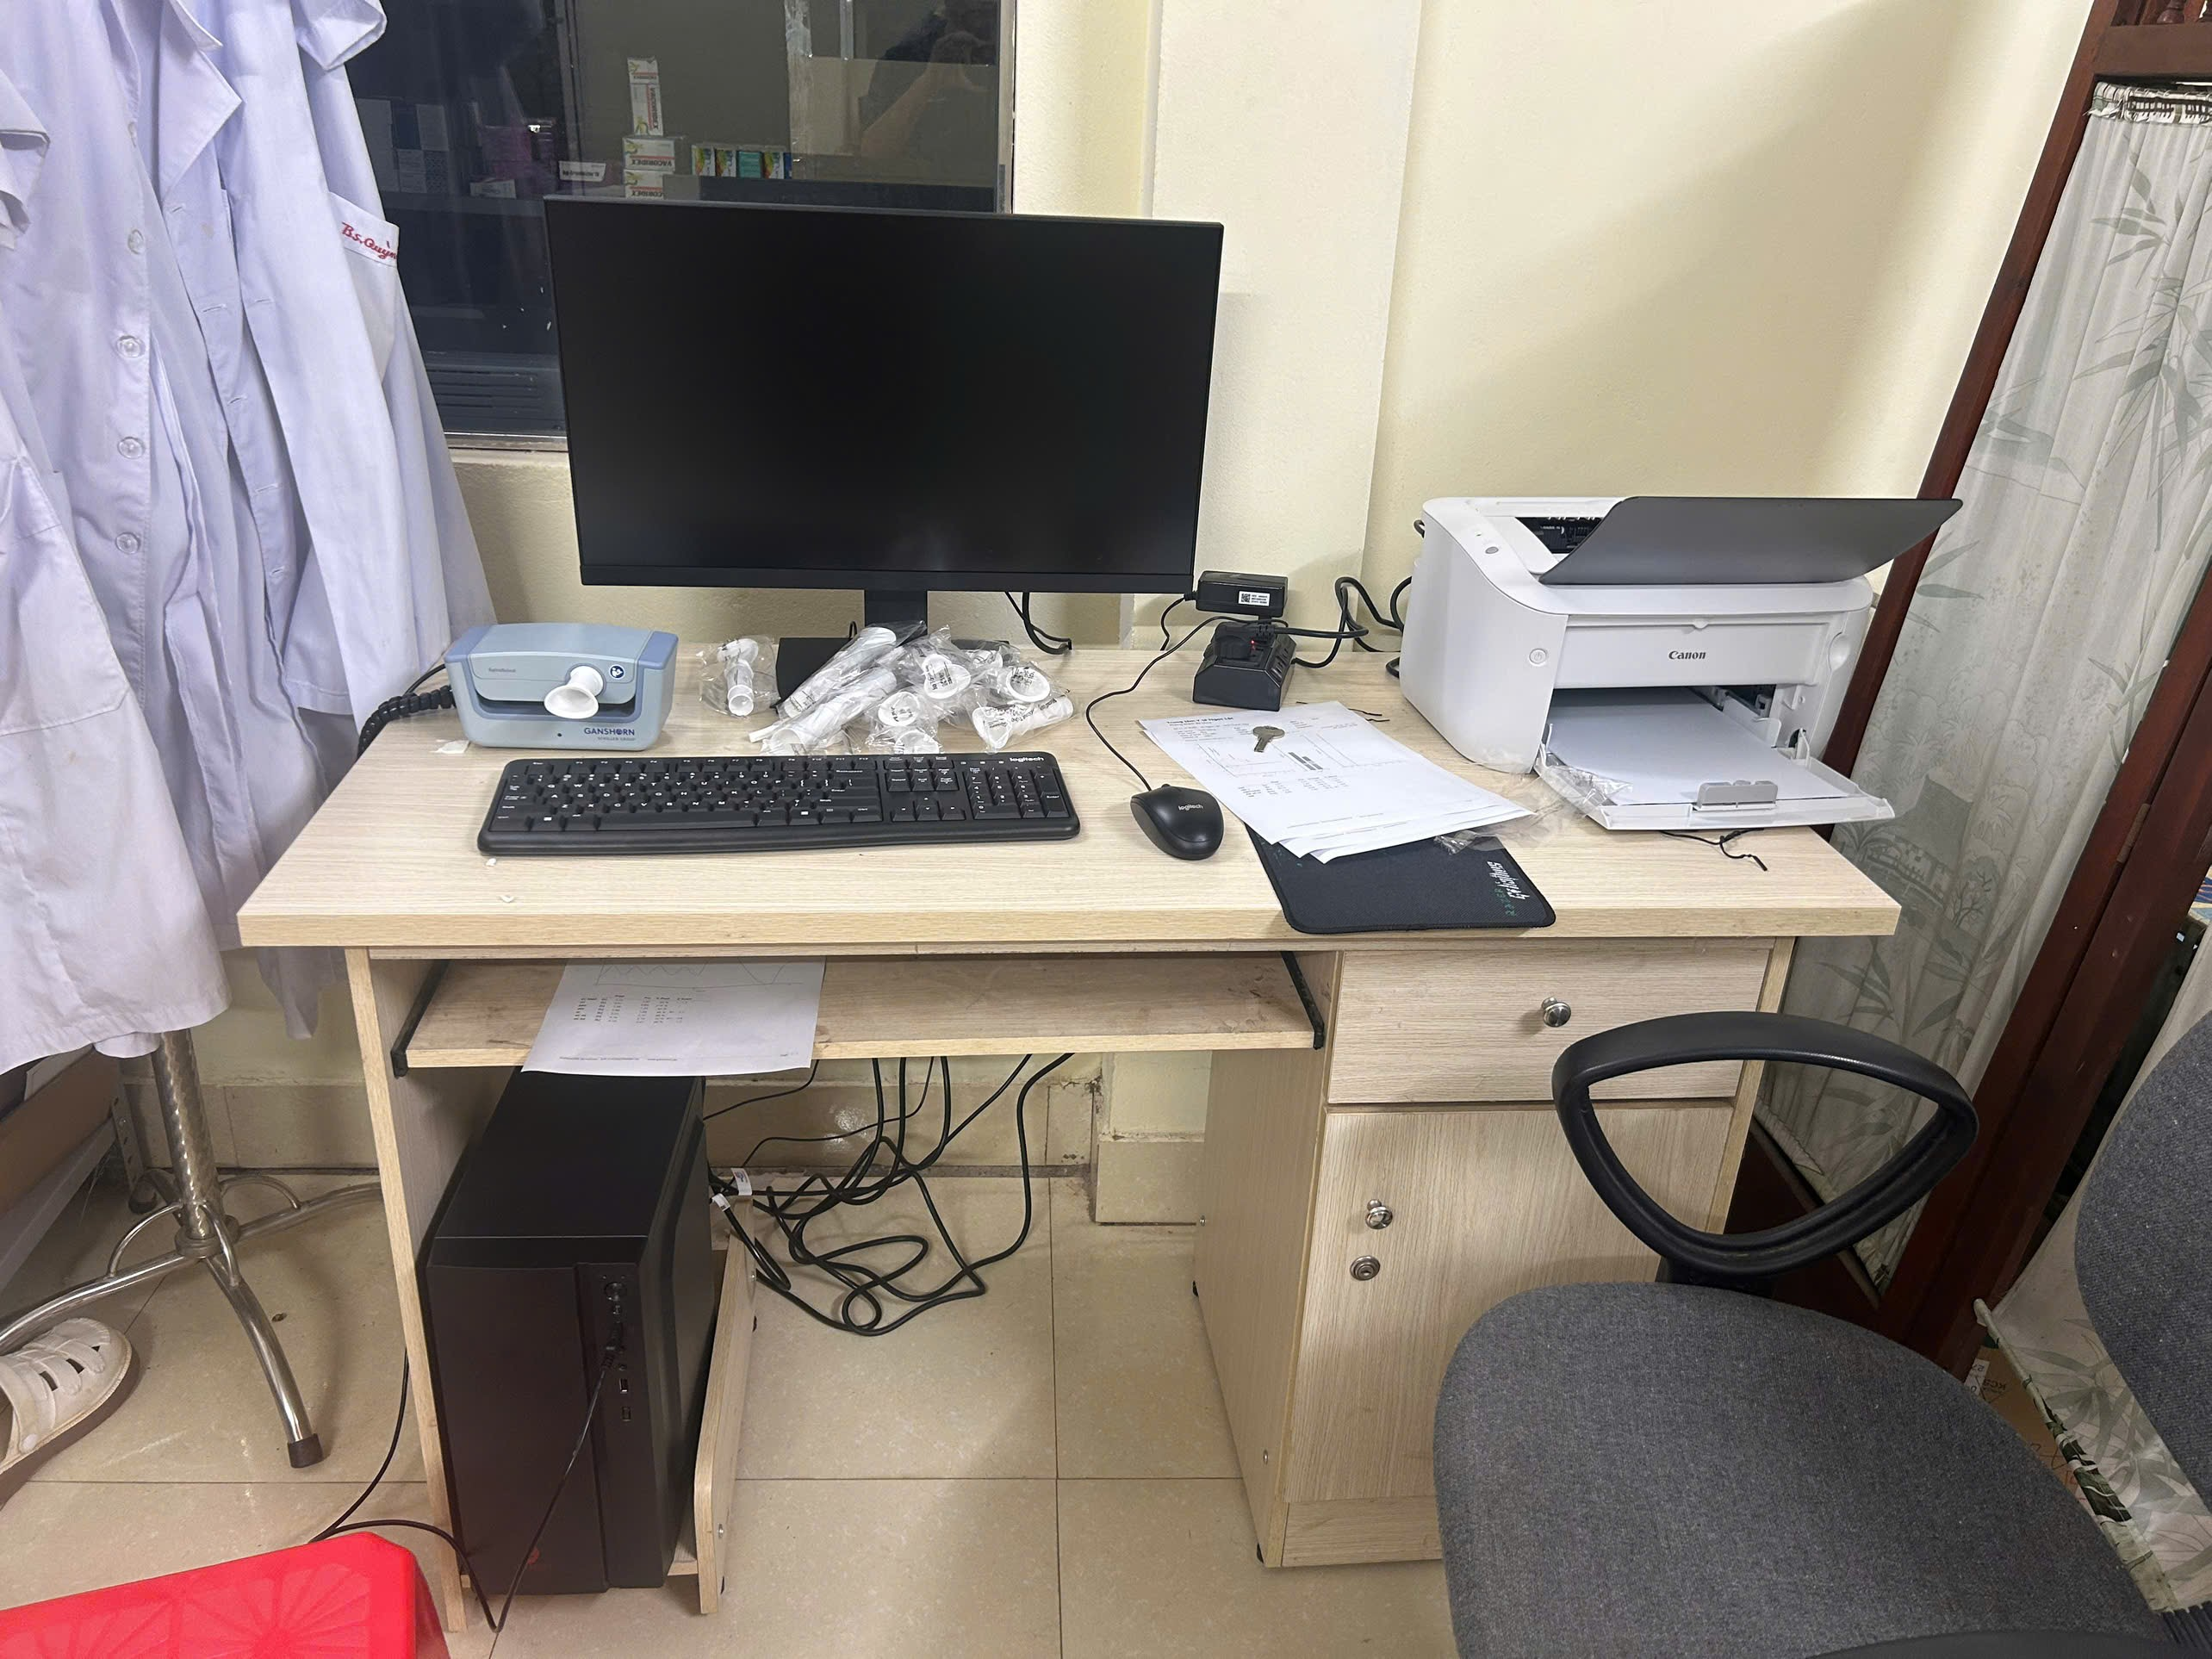
\includegraphics[width=0.5\linewidth]{PC-system.png}
    \caption{Hình ảnh thực tế máy tính trạm ở Trung tâm Y Tế Huyện Ngọc Lặc - Thanh Hoá - Việt Nam}
    \label{fig:placeholder}
\end{figure}

\begin{tabular}{ll}
    \toprule
    Thông số kỹ thuật của PC & \\
    \midrule
    An toàn    & Tuân thủ tiêu chuẩn IEC 60950-1 \\
     Hệ thống vận hành & Windows 7 Professional, 64-bit hoặc 32-bit\\
     Bộ xử lý  & Bộ xử lý tương thích Intel Core i5, 4.0 GHz\\
     Hiệu năng & 1.0 (4.0)\\
     RAM & 4 GB \\
     Bộ nhớ & 5 GB\\
     Độ phân giải màn hình & 1248 x 728\\
     Giao tiếp & USB \\
     \bottomrule
\end{tabular}

\subsection{Phần mềm LPX}

\begin{tabular}{ll}
    \toprule
    %Thông số kỹ thuật phần mềm cho Windows 32 hoặc 64 bit \\
    %\midrule
    Phân loại &  \\
    \midrule
    Thiết bị & Thiết bị y tế chủ động, loại IIa\\
    Phần ứng dụng & Type BF \\
    \midrule
    Hiệu chỉnh & \\
    \midrule
    F/V & ERS hoặc ATS \\
    Hít vào (Inhalation) & BTPS (modun môi trường) hoặc hiệu chỉnh BTPS thời gian thực \\
    Thể tích khí & STPD ( modun môi trường ) hoặc hiệu chỉnh BTPS thời gian thực \\
    \midrule
    Kết nối máy tính\\
    \midrule
    Dữ liệu tới PC & USB 2.0\\
    USB kết nối & Đầu nối A–đầu nối B / dây đôi bọc chống nhiễu / 2 x AWG24,  2 x AWG28\\
    Truyền tín hiệu & Cách ly quang 4 kV RS232, 57.600 Baud\\
    \midrule
    Dữ liệu\\
    \midrule
    Local & Ganshorn SQL\\
     & Xác thực do người dùng định nghĩa \\
     GDT & Nhập và xuất với các cài đặt do người dùng định nghĩa\\
     SEMA3 & tích hợp SCHILLER SEMA3\\
     \midrule
     Đo lưu lượng\\
     \midrule
     Nguyên lý đo & Đo thời gian truyền sóng siêu âm\\
     Khoảng đo & 0 đến +20 l/s\\
     Độ chính xác & < ±2 \% \\
     Độ phân giải & 1 ml \\
     \midrule
     Giá trị đo & \\
     \midrule
      & FEV 1 [L] \\
       & ... \\
    \bottomrule
    
\end{tabular}

\subsection{SpiroScout}

\begin{figure}[H]
    \centering
    \includegraphics[width=0.5\linewidth]{Kích-thước-tổng-quát.png}
    \caption{General dimension}
    \label{fig:placeholder}
\end{figure}

\begin{itemize}
    \item Cảm biến Scout cầm tay với bộ lọc thở dùng một lần: ScoutSensor cầm tay có một miếng đệm thở dùng một lần có thể tháo rời. Trong một số trường hợp lắp đặt, bộ lọc vi khuẩn xài một lần được sử dụng bộ chuyển đổi hình tròn khác.
    \item Base station: Trạm cơ sở cung cấp nền tảng an toàn cho SpiroScout khi không sử dụng và cũng được trang bị hệ thống điều khiển điện tử và các cảm biến để đo điều kiện môi trường xung quanh.
\end{itemize}
\begin{figure}[H]
    \centering
    \includegraphics[width=0.5\linewidth]{SpiroScout.png}
    \caption{SpiroScout}
    \label{fig:placeholder}
\end{figure}

\begin{tabular}{ll}
\toprule
    Thông số kỹ thuật của cảm biến SpiroScout\\
    \midrule
    General &  \\
    \midrule
    Kích thước & 18 cm x 9 cm x (W x H x D)\\
    \addlinespace
    Cân nặng & 1000g (ScoutSensor 185g, Trạm cơ sở 730g, dây 85g)\\
    \addlinespace
    Trở kháng hô hấp & 0.02 kPa/l/s = xấp sỉ 0.02 cmH20/l/s\\
    \addlinespace
    Dead space, complete & 18 cm3\\
    \addlinespace
    Chất liệu & Polythylene\\
    \midrule
    Bảo vệ và vệ sinh bệnh nhân & Chỉ dùng cho bệnh nhân, dùng một lần \\
         & Ống thở SpiroScout, Spirette™ với ống ngậm định hình công thái học và chóp tiêu chuẩn 22 mm, hoặc\\
         &  Bộ lọc vi khuẩn PFT GANSHORN\\
    \midrule
    Nguồn cấp & \\
    \midrule
    Tiêu chuẩn & Cấp nguồn qua USB 2.0 \\
     & Điện áp 4.5 đến 5.25 V DC\\
     & Dòng: 500 mA\\
     \midrule
     Cài đặt nguồn & Bộ đổi nguồn AC bên ngoài \\
     \midrule
     Thông số kỹ thuật của bộ đổi nguồn AC & EGSTON P2CFMW 6 Watt, 5 VDC\\
      & Đầu nối phụ MP205 (tiêu chuẩn y tế). Tiếp điểm bên trong = nối đất, ngoài =+5 VDC,\\
       & Protection class II\\
        & Phạm vi điện áp 100 đến 240 V, 50 đến 60 Hz,\\
    \midrule
    Sự tiêu thụ năng lượng & Chế độ chờ: 275 mA, 5 VDC (1.4 W),\\
     & Chế độ đo: 500mA, 5 VDC (2.5 W)\\
    \bottomrule
\end{tabular}
\subsection{ScoutTube - FPT Filter}

\begin{figure}[H]
    \centering
    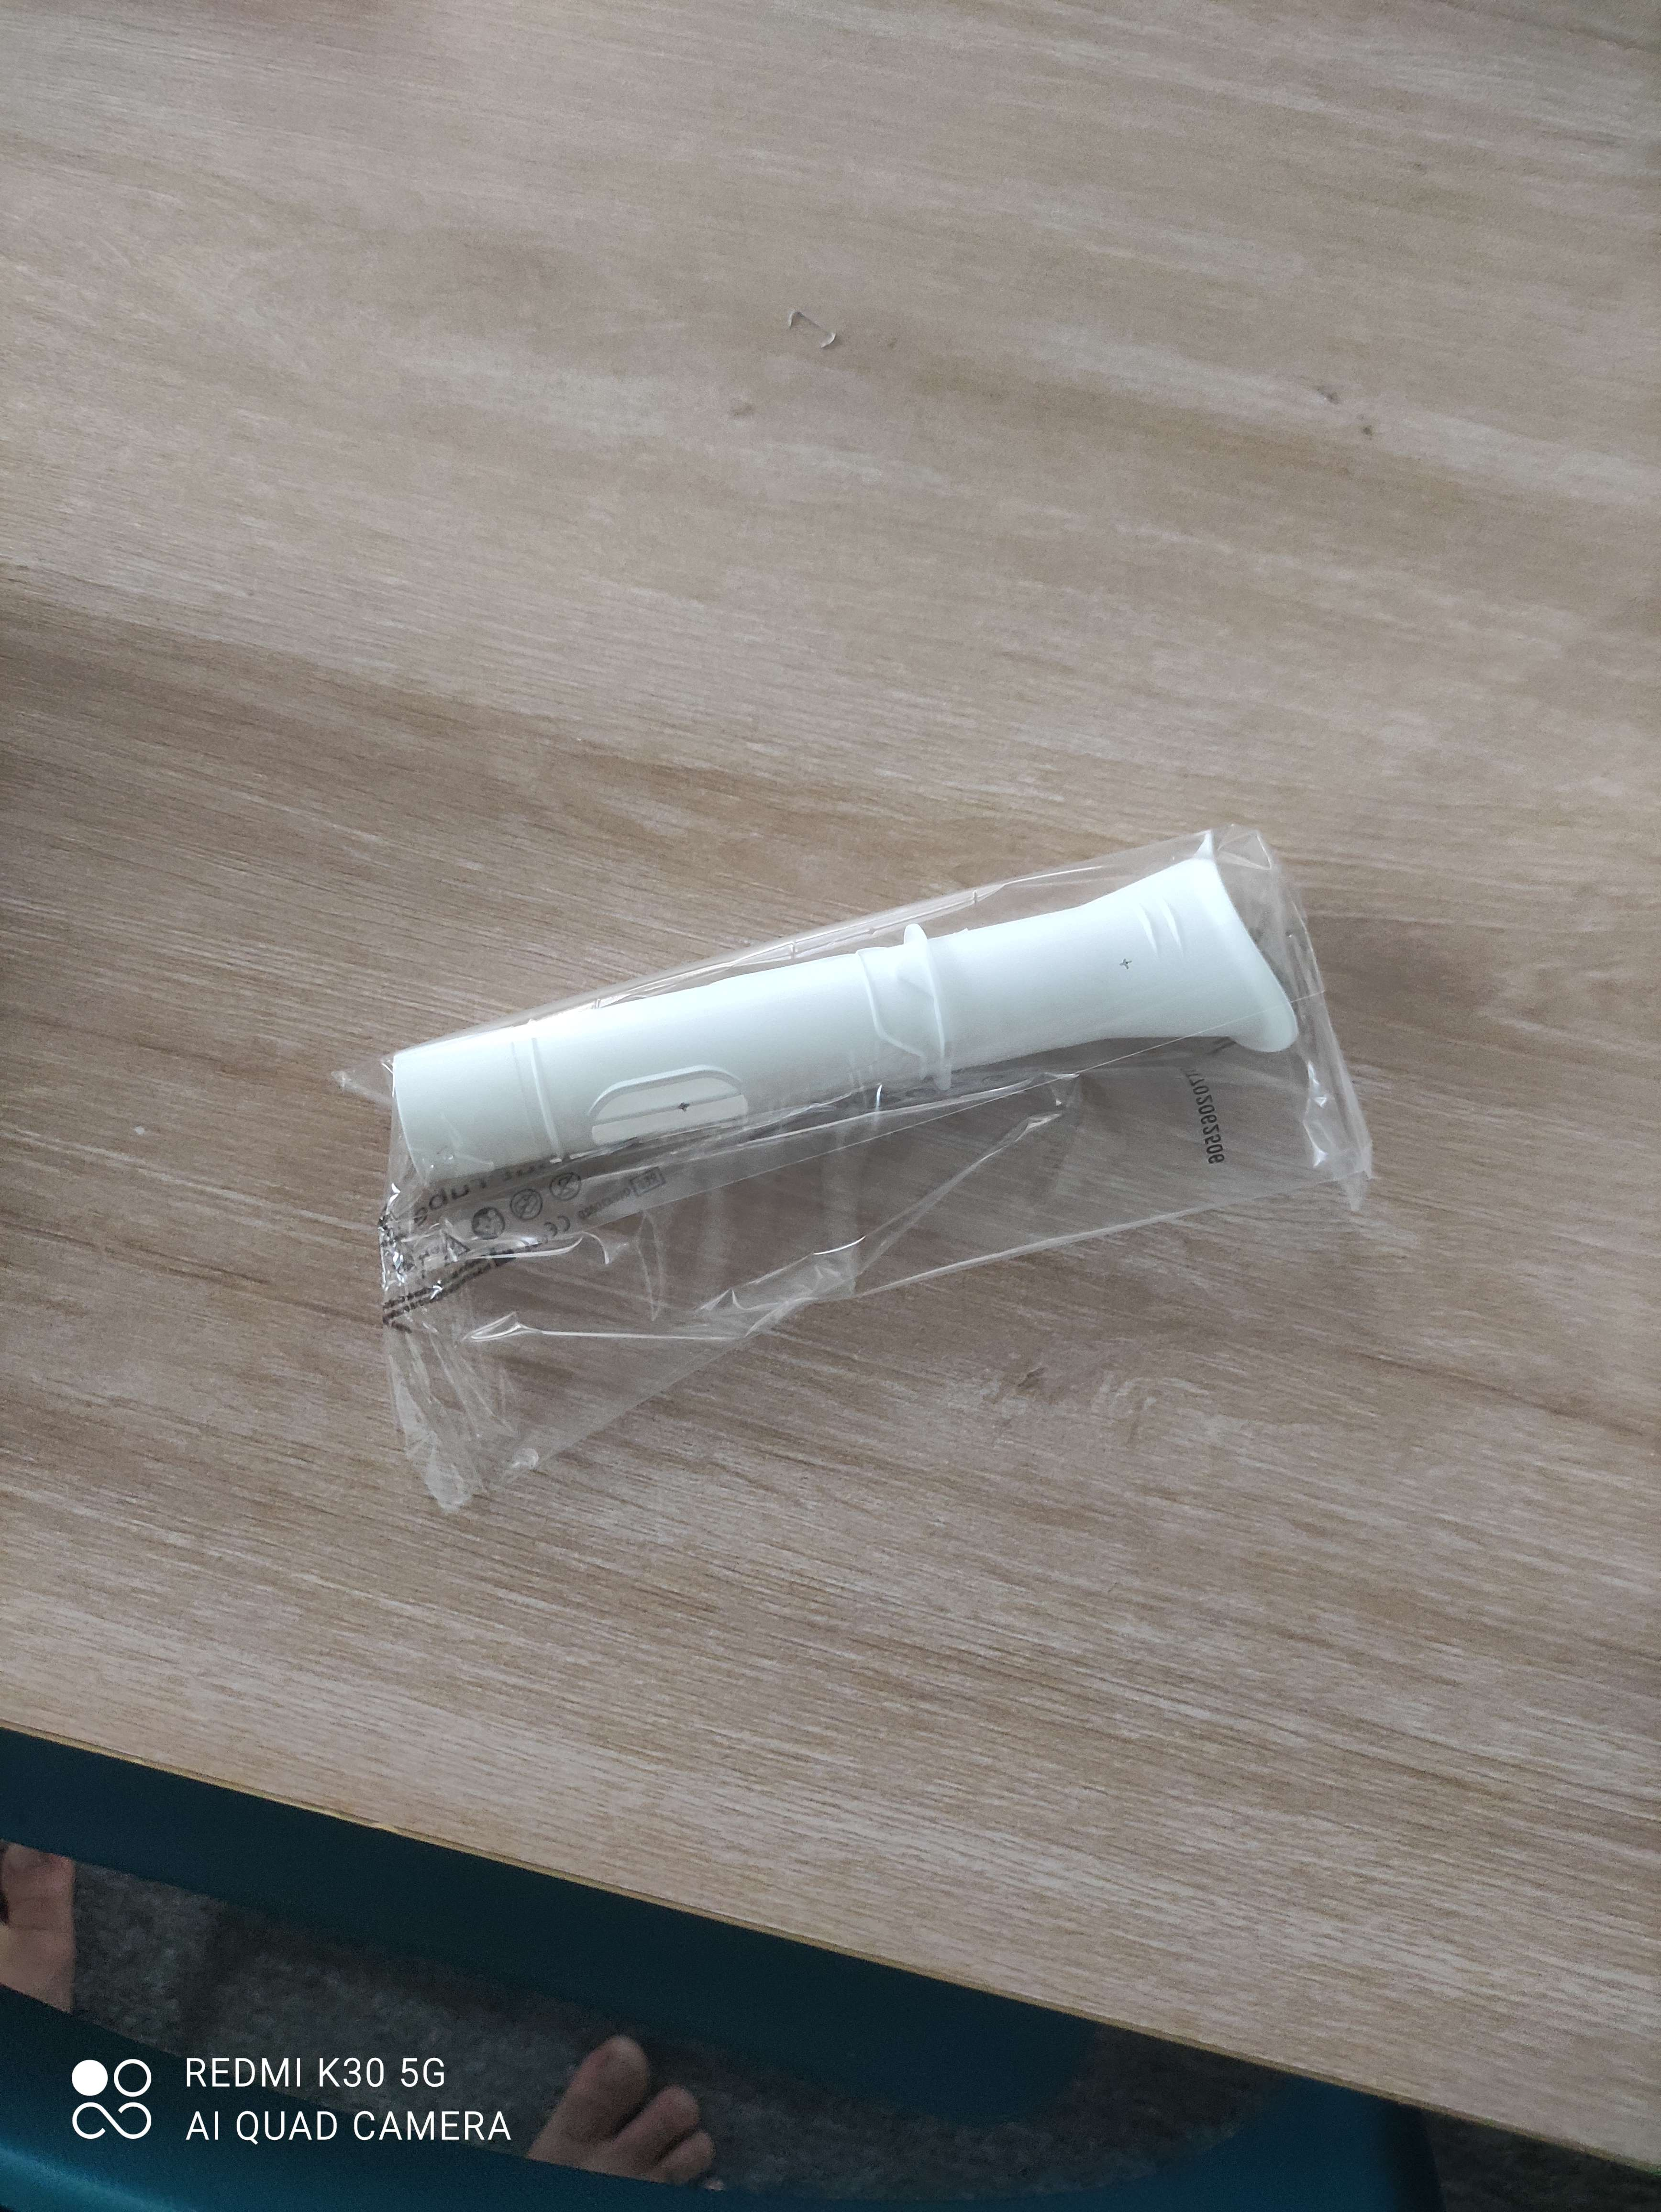
\includegraphics[width=0.5\linewidth]{Real-ScoutTube.png}
    \caption{Hình ảnh thực tế ống lọc PFT}
    \label{fig:placeholder}
\end{figure}

\begin{tabular}{ll}
\toprule
    Thông số kỹ thuật của FPT Filter:\\
    \midrule
   Nhà máy sản xuất  & GANSHORN PTF Filter \\
   \addlinespace
   Loại  & Electrostatic filter, fleece with protective membrane.\\
   \addlinespace
   Bảo vệ vi khuẩn / virus & 99.9999 \% hiệu quả lọc vi khuẩn/virus\\
   \addlinespace
   Sự thoải mái của bệnh nhân & Ống ngậm có hình dáng tiện dụng và hình nón tiêu chuẩn 22 mm \\
   \addlinespace
   Chất liệu & Polypropylen trắng\\
   \addlinespace
   Trở kháng & @ 12 L/s 0.7 cmH20/L/s (0.07 kPa/L/s)\\
   \addlinespace
   Khoang khí chết hiệu dụng & 50 ml\\
   \addlinespace
        & Bộ lọc PFT đáp ứng đầy đủ các khuyến nghị mới nhất từ cả Hiệp hội Hô hấp lồng ngực Hoa Kỳ và Châu Âu (ATS \& ERS)\\
        \addlinespace
    \bottomrule
\end{tabular}

\subsection{Đầu nối, bộ điều khiển và chỉ báo SpiroScout}

\begin{figure}[H]
    \centering
    \includegraphics[width=0.5\linewidth]{SpiroScout-anh2.png}
    \caption{Mặt trước SpiroScout}
    \label{fig:placeholder}
\end{figure}
\begin{figure}[H]
    \centering
    \includegraphics[width=0.5\linewidth]{SpiroScout-anh3.png}
    \caption{Mặt sau SpiroScout}
    \label{fig:placeholder}
\end{figure}

\section{Phần mềm LFX}

Như đã nói ở trên, phần mềm LFX (Lung Function Xperience) là nền tảng phần mềm chuyên dụng được phát triển bởi hãng Garnshorn, hoạt động trên hệ điều hành Windows để điều khiển và vận hành thiết bị SpiroScout. Phần mềm đóng vai trò trung tâm trong việc thu thập tín hiệu thời gian thực từ đầu đo siêu âm, xử lý dữ liệu thô và chuyển đổi thành các biểu đồ, chỉ số lâm sàng có ý nghĩa.\\
\\Với giao diện đồ họa trực quan và hiện đại, LFX được thiết kế để tối ưu hóa quy trình làm việc tại phòng khám, giúp kỹ thuật viên dễ dàng thao tác từ khâu nhập liệu bệnh nhân đến khi xuất báo cáo kết quả.

\begin{figure}[H]
	\centering
	\includegraphics[width=0.5\linewidth]{screen_LFX.png}
	\caption{Màn hình khởi động chương trình LFX}
	\label{fig:screenLFX}
\end{figure}
\subsection{Nhập dữ liệu}

\begin{figure}[H]
	\centering
	\includegraphics[width=0.5\linewidth]{Nhapdulieu.png}
	\caption{Màn hình nhập dữ liệu bệnh nhân}
	\label{fig:placeholder}
\end{figure}
Để đo được kết quả chính xác, người sử dụng cần nhập chính xác các thông tin sau của bệnh nhân: Ngày tháng năm sinh, chiều cao, cân nặng của bệnh nhân, giới tính và cuối cùng là dân tộc. Phần mềm sẽ dựa trên các thông số trên để tính toán các giá trị dưới đây.

\subsection*{Giá trị tính toán của bệnh nhân}
\begin{table}[H]
	\centering
	\small % Dùng font nhỏ hơn một chút để bảng thoáng hơn
	\renewcommand{\arraystretch}{1.5} % Tăng khoảng cách giữa các dòng
	% Cấu trúc: Cột 1 (3cm), Cột 2 (4cm), Cột 3 (Tự động dãn hết phần còn lại)
	\begin{tabularx}{\textwidth}{|p{3cm}|p{4cm}|X|}
		\hline
		\textbf{Giá trị tính toán} & \textbf{Giải thích} & \textbf{Công thức} \\
		\hline
		
		BSA & Diện tích bề mặt cơ thể tính bằng $m^2$ theo Mosteller & 
		\begin{itemize}[nosep, leftmargin=1em, label=\textbullet, before=\vspace*{-\baselineskip}, after=\vspace*{-\baselineskip}]
			\item Công thức dành cho nam và nữ:
			
			\item $BSA = \sqrt{\frac{\text{Chiều cao (cm)} \times \text{Cân nặng (kg)}}{3600}}$
		\end{itemize} \\
		\hline
		
		
		BMI & Chỉ số khối cơ thể tính bằng $kg/m^2$ theo Adolphe Quetelet & 
		\begin{itemize}[nosep, leftmargin=1em, label=\textbullet, before=\vspace*{-\baselineskip}, after=\vspace*{-\baselineskip}]
			\item Công thức dành cho nam và nữ:
			\item $BMI = \frac{\text{Cân nặng (kg)}}{\text{Chiều cao}^2 (m)}$
		\end{itemize} \\
		\hline
		
		Cân nặng lý tưởng (Ideal weight) & Cân nặng lý tưởng tính bằng kg theo Dr. Devine & 
		\begin{itemize}[nosep, leftmargin=1em, label=\textbullet, before=\vspace*{-\baselineskip}, after=\vspace*{-\baselineskip}]
			\item \textbf{Nam:} $50 + 2,3$ kg cho mỗi inch trên 5 feet.
			\item \textbf{Nữ:} $45,5 + 2,3$ kg cho mỗi inch trên 5 feet.
		\end{itemize} \\
		\hline
		
		Trọng lượng tương đối (Rel. weight) & Trọng lượng tương đối tính bằng \% & 
		\begin{itemize}[nosep, leftmargin=1em, label=\textbullet, before=\vspace*{-\baselineskip}, after=\vspace*{-\baselineskip}]
			\item Công thức dành cho nam và nữ:
			\item $\text{TL tương đối} = \frac{\text{Cân nặng (kg)}}{\text{Chiều cao (cm)} - 100} \times 100$
		\end{itemize} \\
		\hline
		
		LBW & Trọng lượng cơ thể nạc tính bằng kg theo James & 
		\tabitem \textbf{Nam:} $LBW = (1.10 \times \text{Cân nặng}) - 128 \times (\frac{\text{Cân nặng}}{100 \times \text{Chiều cao}})^2$ \newline
		\tabitem \textbf{Nữ:} $LBW = (1.07 \times \text{Cân nặng}) - 148 \times (\frac{\text{Cân nặng}}{100 \times \text{Chiều cao}})^2$ \\
		\hline
		
		Chiều cao từ khoảng cách cánh tay & Công thức dùng ước tính chiều cao bệnh nhân & 
		\tabitem \textbf{Tuổi < 18 (Hibbert, Torres):} \newline 
		$\text{Chiều cao (cm)} = \text{Sải tay (cm)}$ \newline
		\tabitem \textbf{Tuổi > 18 (Parker và cộng sự):} \newline
		$\text{Chiều cao} = 67,90 + 0,664182 \times \text{Sải tay} + 2,816 \times \text{Giới tính} - 4,05 \times \text{Chủng tộc} - 0,0709 \times \text{Tuổi}$ \newline
		\textit{(Trong đó: Giới tính: 1=Nam, 2=Nữ; Chủng tộc: 1=Trắng, 2=Đen)} \\
		\hline
		
		Pack years (Hút thuốc) & Công thức tính số năm hút thuốc & 
		\tabitem $\text{Năm} = \frac{\text{Thuốc lá mỗi ngày}}{\text{Thuốc lá mỗi gói}} \times \text{Số năm hút thuốc}$ \\
		\hline
	\end{tabularx}
\end{table}

\section{Nguyên lý đo lường}
Máy SpiroCount sử dụng công nghệ đo lưu lượng bằng cảm biến siêu âm (Ultrasonic Flow Measurement) thay vì sử dụng tuabin quay hay cảm biến chênh áp truyền thống. Nguyên lý hoạt động dựa trên sự thay đổi thời gian truyền của sóng âm khi đi qua dòng khí đang chuyển động.
\section*{Cấu tạo cảm biến}
Hệ thống đo lượng bao gồm một ống thở và hai đầu dò siêu âm được bố trí đối diện nhau theo một đường chéo cắt ngang dòng khí.
\begin{figure}[H]
    \centering
    \includegraphics[width=0.5\linewidth]{measurement-principle.png}
    \caption{Cảm biến lưu lượng siêu ẩm}
    \label{fig:placeholder}
\end{figure}

\section*{Quy trình đo lường}
Quá trình xác định lưu lượng khí thở diễn ra theo các bước sau:
\begin{enumerate}
	\item \textbf{Phát -- Thu tín hiệu:} Hai đầu dò siêu âm hoạt động luân phiên, vừa là bộ phát vừa là bộ thu. Chúng liên tục gửi các xung sóng siêu âm qua lại cho nhau: một xung đi xuôi theo chiều dòng khí và một xung đi ngược chiều dòng khí.
	
	\item \textbf{So sánh thời gian truyền (Transit-time):}
	\begin{itemize}
		\item \textbf{Khi không có dòng khí (Lưu lượng = 0):} Thời gian truyền sóng của hai hướng là bằng nhau.
		\item \textbf{Khi bệnh nhân thở (Có dòng khí):} Dòng khí sẽ làm tăng tốc độ sóng âm đi "xuôi dòng" và làm chậm tốc độ sóng âm đi "ngược dòng".
	\end{itemize}
	
	\item \textbf{Tính toán kết quả:}
	\begin{itemize}
		\item Máy sẽ đo sự chênh lệch thời gian ($\Delta t$) giữa hai xung sóng. Sự chênh lệch này tỷ lệ thuận trực tiếp với vận tốc của dòng khí.
		\item Từ vận tốc dòng khí và tiết diện ống thở, bộ vi xử lý sẽ tính toán ra \textbf{Lưu lượng (Flow)} và \textbf{Thể tích (Volume)} khí thở của bệnh nhân.
	\end{itemize}
\end{enumerate}


\section{Quy trình vận hành}
\subsection{Quá trình lắp đặt và chuẩn bị ban đầu}
\begin{enumerate}
	\item{Kết nối SpiroCount với PC}
	\begin{enumerate}
		\item Đảm bảo PC đã tắt.
		\item Tại SpiroScout, kết nối cáp cảm biến giữa đầu nối RS232 trên Cảm biến và đầu nối RS232 trên đế.
		\item Sử dụng cáp USB để truyền dữ liệu với PC. Đầu nối cổng USB ở trạm gốc với cổng USB miễn phí trên PC.
		\item Nếu hệ thống của bạn được cung cấp bộ chuyển đổi AC riêng, hãy kết nối bộ chuyển đổi AC với ổ cắm DC-IN.
	\end{enumerate}
	
	\item{Khởi động hệ thống}
	\begin{enumerate}
		\item Bật PC
		\item Bật SpiroScout bằng công tắc nguồn ở phía sau trạm gốc.\\ Kiểm tra xem đèn báo nguồn ở mặt trước của bộ phận đế có sáng đỏ hay không.Tín hiệu được đưa ra khi bật lần đầu tiên. Điều này cho thấy SpiroScout đã sẵn sàng để sử dụng.
		\item Khởi động chương trình LFX từ màn hình nền Windows bằng cách nhấp đúp vào biểu tượng LFX.
	\end{enumerate}
\end{enumerate}
\subsection{Lắp bộ lọc thở PFT dùng một lần}
\begin{enumerate}
	\item Dụng cụ thở dùng một lần
	\begin{itemize}
		\item Ống thở SpiroScout (SpiretteTM) là vật dụng dùng một lần và không được tái sử dụng. Một cái mới phải được sử dụng cho mỗi bệnh nhân. Không sử dụng cho nhiều hơn một bệnh nhân.
		\item Không cố gắng làm sạch
	\end{itemize}
	\begin{figure}[H]
		\centering
		\includegraphics[width=0.5\linewidth]{setting-PFT-filter.png}
		\caption{Lắp đặt ống thở lọc khuẩn PFT}
		\label{fig:placeholder}
	\end{figure}
	\item Tháo miếng đệm thở
	Để tháo miếng đệm thở, hãy kéo nó ra khỏi giá đỡ ScoutSensor, xoay nó ngược chiều kim đồng hồ một chút nếu cần.
	\item Lắp bộ lọc vi khuẩn PFT
	\begin{itemize}
		\item Chỉ sử dụng một lần - không sử dụng bộ lọc PFT cho nhiều bệnh nhân.
		\item Không cố gắng làm sạch bộ lọc.
		\item Chỉ sử dụng bộ lọc vi khuẩn được GANSHORN phê duyệt. Việc sử dụng bất kỳ bộ lọc nào khác có thể gây ra kết quả đo không chính xác.
	\end{itemize}
	Bộ lọc vi khuẩn là bộ lọc vi khuẩn sử dụng một lần được thiết kế để giúp giảm thiểu nguy cơ ô nhiễm không khí và nguy cơ lây nhiễm chéo khi thực hiện các xét nghiệm chức năng phổi và vừa khít với ống ngậm để tạo thành một miệng bịt kín khí.\\
\end{enumerate}
\section*{Kiểm tra trong suốt quá trình lắp đặt}
\begin{itemize}
	\item Quan sát tất cả các quy trình lây nhiễm chéo, ví dụ: đeo găng tay cao su, không để chất thải y tế tiếp xúc với bất kỳ ai, loại bỏ và vứt bỏ màng lọc vi khuẩn vào trong chất thải y tế.
	\item Lau/làm sạch ScoutSensor bằng dung dịch làm sạch hoặc chất khử trùng đã được phê duyệt
\end{itemize}
\subsection{Làm sạch và khử trùng}
SpiroScout và bộ phận đế có thể được lau bằng vải ẩm để làm sạch. Có thể sử dụng chất khử trùng tiêu chuẩn của bệnh viện để khử trùng SpiroScout.
Cảm biến siêu âm phải được khử trùng hằng tuần.

\subsection{Xác minh và hiệu chỉnh}
SpiroScout kết hợp các cảm biến áp suất và độ ẩm,  và vì SpiroScout hoạt động dựa trên việc đo thời gian truyền sóng âm nên việc hiệu chuẩn thể tích hằng ngày là hoàn toàn không cần thiết. Hiện tại thiết bị chỉ cần hiệu chỉnh điểm 0, một số tham số phụ của môi trường bên ngoài, và thể tích theo yêu cầu của tiêu chuẩn quốc tế 
\subsubsection{Hiệu chuẩn điểm 0}
Hiệu chuẩn điểm 0 được thực hiện tự động khi bật nguồn và sau 15 phút mỗi lần. Trong quá trình điều chỉnh về 0, máy xác định trạng thái "tĩnh" của dòng khí trong ống đo để thiết lập mức tham chiếu. Lưu ý:
\begin{itemize}
	\item Không di chuyển cảm biến.
	\item Không thở vào cảm biến.
	\item Ngăn gió lùa vào, đóng cửa sổ phòng, và không di chuyển bất kỳ bộ phận nào của thiết bị.
\end{itemize}
\subsubsection{Thông số môi trường xung quanh}
Dựa trên các giá trị được hệ thống đo trực tiếp, nhiệt độ $[^\circ C]$ và áp suất xung quanh $[hPa]$, cũng như các giá trị được cài đặt thủ công, độ ẩm $[\%]$ và độ cao so với mực nước biển $[m]$, các thông số môi trường này cần được cập nhập theo định kỳ để đảm bảo phép đo chính xác nhất, chương trình LFX xác định hệ số điều chỉnh thể tích STPD và BTPS.\\
Trong đó:
\begin{itemize}
	\item BTPS (Body Temperature, Pressure, Saturated): 
	Đây là điều kiện khí bên trong cơ thể (phổi) của con người. 
	\begin{itemize}
		\item Body Temperature: Nhiệt độ cơ thể, thường lấy ở $37^\circ C$ hay 310K.
		\item Pressure: Áp suất khí quyển tại nơi đo.
		\item Saturated: Bão hoà hơi nước (độ ẩm $100\%$ tại $37^\circ C$, áp suất hơi nước khoảng 47 mmHg).
	\end{itemize}
	\item STPD (Standard Temperature, Pressue, Dry): Điều kiện khí tiêu chuẩn, thường dùng trong các nghiệm pháp gắng sức tim mạch - hô hấp, để đo sự tiêu thụ $O_2$ hoặc thải $CO_2$.
\end{itemize}
\subsubsection{Hiệu chuẩn thể tích}
Để đảm bảo độ tin cậy cho hệ thống, và tuân thủ các tiêu chuẩn quốc tế, thể tích có thể được hiệu chuẩn theo các yêu cầu dưới đây:
\begin{itemize}
	\item Chỉ sử dụng ống tiêm hiệu chuẩn ban đầu và bộ chuyển đổi silicon do GANSHORN cung cấp hoặc phê duyệt. Ống tiêm hiệu chuẩn phải được xác minh thường xuyên.
	\item Việc xác minh và hiệu chuẩn thể tích được thực hiện bằng ống tiêm hiệu chuẩn được kết nối với cảm biến và xả/sạc ở tốc độ ổn định với phạm vi lưu lượng trong khoảng từ 0.5 đến 1.2 lít trên giây.
	\item Kết quả đo được phải nằm trong sai số $\pm 3.5\%$ (bao gồm cả độ chính xác $0.5\%$ của ống tiêm). 
\end{itemize}
\subsubsection{Quy trình hiệu chuẩn thể tích}
\begin{enumerate}
	\item Lắp ống thở mới hoặc đặt bộ lọc vi khuẩn PFT mới vào cảm biến.
	\item Từ màn hình bệnh nhân, nhấp vào nút Calib.
	\item Cài đặt hiệu chỉnh được hiển thị ở bên phải màn hình.
	\item Nhấp vào Vol để vào màn hình hiểu chuẩn.
	\item Nhập thể tích của ống tiêm hiệu chuẩn (Nên dùng ống tiêm 3 lít).
	\item Kết nối ống tiêm hiệu chuẩn với bộ chuyển đổi silicon và bộ lọc PFT.
	\item Đảm bảo tiếp xúc tốt và không rò rỉ.
	\item Nhấp vào nút bắt đầu.\\
	Một thông báo hiện ra: \textit{Calibrating Offset. Please don’t breathe or create any flow in front of the sensor}
	\item Sau một lúc, độ lệch được hiệu chỉnh và màn hình hiển thị thể tích hiện lên. Kéo piston nhẹ nhàng qua lại với lưu lượng không đổi từ 0.5 đến 12 L/s.
	\item Sau vài lần bơm, chương trình sẽ tự động dừng và hiện thị thông báo thành công hoặc thất bại.
\end{enumerate}
\begin{figure}[H]
	\centering
	\includegraphics[width=0.5\linewidth]{volume_calibration.png}
	\caption{Màn hình hiệu chuẩn thể tích}
	\label{fig:volume_calibration}
\end{figure}
\subsubsection{Kết quả dạng bảng sau khi hiệu chuẩn}
Thể tích sau khi hiệu chuẩn sẽ được hiển thị trong kết quả dạng bảng. Thể tích ở mỗi luồng phải đáp ứng yêu cầu về độ chính xác là $3.5\%$ (bao gồm độ chính xác $0.5\%$ của ống tiêm). Đối với ống tiêm 3 lít, thể tích đo được ở mỗi lần bơm phải nằm trong khoảng 2.895 và 3.105 lít.\\
Chúng ta có thể tăng tốc độ dòng từ 0.5 L/s lên 6L/s rồi 12L/s để kiểm tra độ tuyến tính của cảm biến lưu lượng.
\subsection{Kết quả tốt nhất và giá trị dự đoán}
Theo tiêu chuẩn đo phế dung của Hiệp hội Lồng ngực Hoa Kỳ (ATS) (ngày 11 tháng 11 năm 1994), phép đo tốt nhất được xác định là giá trị cao nhất từ phép tính:
$$\text{Best} = \text{FVC} + \text{FEV1(or FEV6)}$$
Chương trình đo phế dung lấy giá trị tốt nhất được xác định ở trên và xác định giá trị này là 'lựa chọn ưu tiên'  theo khuyến nghị của ATS và ERS.
\subsection{Tổng quan phép đo}
\subsubsection{Đo phế dung chậm}
Đo phế dung chậm được thực hiện để đo thể tích phổi hít vào và thở ra (SVC, VCin, VCex, ERV, IC, v.v.v.) trong các thao tác chậm. Nó đo lượng không khí một người hít vào và thở ra theo thời gian.\\
Nên thực hiện các thao tác VC trước các thao tác FVC vì có khả năng xảy ra tắc nghẽn phế quản hoặc giãn phế quản sau khi thực hiện các thao tác cưỡng bức.\\
Trong quá trình thực hiện thủ thuật này, bệnh nhân nên thở bình thường 3 lần rồi hít vào càng nhiều càng tốt cho dung tích phổi tối đa, sau đó thở ra hết sức có thể.
\subsubsection*{Thông số đo}
Dung tích sống (VC) có thể đo được bằng cách thực hiện thao tác thở theo 2 cách khác nhau. 

\begin{enumerate}
	\item \textbf{Động tác hít vào gắng sức(IVC maneuverer)}\\
	Sau một thời gian thở nhẹ và đều đặn (thở bình thường), bệnh nhân thở ra hoàn toàn, sau đó hít vào hoàn toàn. IVC(Inspiratory Vital Capacity) là dung tích hít vào, đây là lượng khí tối đa mà một người có thể hít vào sau khi đã thở ra hết sức.
	\begin{figure}[H]
		\centering
		\includegraphics[width=0.5\linewidth]{IVC.png}
		\caption{Giản đồ ghi lại thể tích phổi theo thời gian trong IVC}
		\label{fig:IVC}
	\end{figure}
	\item \textbf{Động tác thở ra gắng sức (EVC maneuverer)}\\
	Sau một thời gian thở nhẹ và đều đặn, bệnh nhân hít vào hoàn toàn, sau đó thở ra hoàn toàn. EVC(Expiratory Vital Capacity) là dung tích khí mà một người có thể thở ra sau khi hít vào hết sức, với tốc độ thở từ từ, không gấp gáp.
	\begin{figure}[H]
		\centering
		\includegraphics[width=0.5\linewidth]{EVC.png}
		\caption{Giản đồ ghi lại thể tích phổi theo thời gian trong EVC}
		\label{fig:EVC}
	\end{figure}
\end{enumerate}
\subsubsection*{Các thông số khác được đo trong quá trình đo Phế dung ký chậm}
\begin{itemize}
	\item BF = Breathing Frequency (1/min) : Số nhịp thở bệnh nhân thực hiện trong một phút.
	\item MV = Minute Volume (L/min) : Là tổng lượng khí được hít vào hoặc thở ra trong một phút. = BF * VT(Thể tích khí lưu thông)
	\item VC MAX = Maximal Vital Capacity (L) : Là giá trị dung tích sống cao nhất ghi nhận được. Máy sẽ tự động so sánh và chọn giá trị lớn hơn giữa $VC_{IN}$ (Dung tích sống hít vào) hoặc $VC_{EX}$ (Dung tích sống thở ra).
	\item T EX = Time expiatory tidal breath (sec). : Thời gian của thì thở ra trong một nhịp thở thường.
	\item T IN = Time inspiratory tidal breath (sec).: Thời gian của thì hít vào trong một nhịp thở thường.
	\item T TOT = Time complete tidal breathing manouvre (sec).: Tổng thời gian để hoàn thành trọn vẹn một chu kỳ thở thường (bao gồm hít vào và thở ra).
	\item TI/TE = Ratio of the T IN and T EX: Tỷ lệ giữa thời gian hít vào ($T_{IN}$) và thời gian thở ra ($T_{EX}$).
\end{itemize}
\subsubsection{Đo phế dung cưỡng bức}
Phép đo phế dung cưỡng bức được thực hiện để đo thể tích và lưu lượng thở ra và hít vào trong quá trình gắng sức tối đa. Nó đo lường cách một người hít vào thở ra mạnh một lượng không khí. Các phép đo chính như sau :
\begin{enumerate}
	\item \textbf{Dung tích sống gắng sức - Forced Vital Capacity (FVC)}: Lượng khí (tính bằng lít) đo được trong quá trình thở ra mạnh và hết sức có thể, bắt đầu từ vị trí hít vào đầy phổi.
	\item \textbf{Thể tích thở ra gắng sức trong giây đầu - The forced expiratory volume in one second (FEV1)}: Lượng khí (tính bằng lít) đo được trong giây đầu tiên của nghiệm pháp thở ra gắng sức.
\end{enumerate}
\subsubsection*{Thông số đo}
Trong quá trình đo phế dung cưỡng bức, chúng ta đo các thông số liên quan đến thể tích và lưu lượng trong các thao tác cưỡng bức.
\begin{enumerate}
	\item \textbf{Các thông số thể tích}: Dung tích sống gắng sức (FVC) và thể tích thở ra gắng sức trong 1s (FEV1) đều được biểu thị bằng lít. Ngoài 2 thông số này, chúng ta còn có thể đo: IRV, VT, ERV và IC. 
	\begin{figure}[H]
		\centering
		\includegraphics[width=0.8\linewidth]{volume.png}
		\caption{Volume related parameters}
		\label{fig:volume}
	\end{figure}
	\item \textbf{Các thông số lưu lượng}: Lưu lượng thở ra tối đa được xác định từ thở ra gắng sức tối đa được gọi là lưu lượng thở ra cao nhất (PEF). Lưu lượng hít vào tối đa (PIF) và lưu lượng hít vào tối đa được xác định từ hít vào tối đa. Ngoài ra, chúng ta cũng có thể đo lưu lượng thở ra ở một thể tích dài cụ thể trong thao tác thở ra gắng sức (VD: MEF75, MEF50, MEF25).
	\begin{figure}[H]
		\centering
		\includegraphics[width=0.8\linewidth]{flow.png}
		\caption{Flow related parameters}
		\label{fig:flow}
	\end{figure}
\end{enumerate}
\subsubsection*{Các thông số khác được đo trong quá trình đo Phế dung cưỡng bức}
\begin{itemize}
	\item FVC IN = Dung tích sống hít vào cưỡng bức(L)
	\item FIV1 = Dung tích hít vào cưỡng bức trong 1s (L)
	\item FIV0.5 = Dung tích hít vào cưỡng bức trong 0.5s (L)
	\item FIV.75 = Dung tích hít vào cưỡng bức trong 0.75s (L)
	\item FIV2 = Dung tích hít vào cưỡng bức trong 2s (L)
	\item FIV3 = Dung tích hít vào cưỡng bức trong 3s (L)
	\item FIV6 = Dung tích hít vào cưỡng bức trong 6s (L)
	\item MMEF = Lưu lượng thở ra tối đa giữa thì (L/s)
	\item VC IN = Dung tích sống hít vào (L)
	\item VC EX = Dung tích sống thở ra (L)
	\item VC MAX = Dung tích sống đo được tối đa (L)
	\item EV = Dung tích thở ra (L)
	\item $\text{EV\%FVC}$ = Dung tích thở ra theo phần trăm của FCV($ \% $).
	\item PEFT = Thời gian cho đến khi đạt lưu lượng thở ra cao nhất (sec).
	\item AEX = Diện tích đường cong thở ra ($L*L/s $)
	\item AIN = Diện tích đường cong hít vào ($L*L/s $)
	\item BF = Tần suất thở (1/min)
	\item MV = Thông khí tối đa (L/min)
	\item T EX =  Thời gian của thì thở ra trong một nhịp thở thường (sec).
	\item T IN = Thời gian của thì hít vào trong một nhịp thở thường.
	\item T TOT =Tổng thời gian để hoàn thành trọn vẹn một chu kỳ thở thường (bao gồm hít vào và thở ra).
	\item TI/TE =Tỷ lệ giữa thời gian hít vào ($T_{IN}$) và thời gian thở ra ($T_{EX}$).
\end{itemize}

\subsubsection{Kiểm soát chất lượng trong quá trình đo}
Tiêu chí kết thúc thử nghiệm đạt được khi: thời gian thở ra là $\ge$ 6 giây (3 giây ở trẻ > 10 tuổi) hoặc khi thể tích < 25 ml trong một giây.
Theo hướng dẫn ATS/ERS 2005, tiêu chí cuối cùng của bài kiểm tra được đáp ứng khi ít nhất đạt được một trong 2 tiêu chí này.
\section{Hình ảnh của một số phép đo}
\subsection{Đo phế dung ký chậm}
\begin{figure}[H]
	\centering
	\includegraphics[width=0.8\linewidth]{SV_review.png}
	\caption{Đang thực hiện đo phế dung ký chậm}
\end{figure}

\begin{figure}[h]
	\centering
	% ---------------- HÀNG 1: HÌNH TRÊN ----------------
	% Cột bên trái: Chứa Caption 1
	\begin{minipage}[c]{0.35\textwidth} 
		\caption{Biểu đồ minh họa quá trình hít vào (IVC). Đường cong đi lên thể hiện dung tích hít vào tối đa.}
		\label{fig:hinh_tren}
	\end{minipage}
	\hfill % Đẩy hình sang phải
	% Cột bên phải: Chứa Hình 1
	\begin{minipage}[c]{0.6\textwidth}
		\centering
		\includegraphics[width=\linewidth]{IVC_review.png} 
	\end{minipage}
	
	% Tạo khoảng cách giữa 2 hình (quan trọng)
	\vspace{1cm} 
	
	% ---------------- HÀNG 2: HÌNH DƯỚI ----------------
	% Cột bên trái: Chứa Caption 2
	\begin{minipage}[c]{0.35\textwidth} 
		\caption{Biểu đồ minh họa quá trình thở ra (EVC). Đường cong đi xuống thể hiện dung tích thở ra tối đa.}
		\label{fig:hinh_duoi}
	\end{minipage}
	\hfill % Đẩy hình sang phải
	% Cột bên phải: Chứa Hình 2
	\begin{minipage}[c]{0.6\textwidth}
		\centering
		\includegraphics[width=\linewidth]{EVC_review.png} 
	\end{minipage}
\end{figure}

\begin{figure}[H]
	\centering
	\includegraphics[width=0.8\linewidth]{SVC_review.png}
	\caption{Kết quả cuối cùng của đo phế dung ký chậm}
\end{figure}
\textbf{Nhận xét}: SVC dùng để xác nhận xem phổi có bị nhỏ đi hay cứng lại không (như trong bệnh xơ phổi, vẹo cột sống, béo phì).
\subsection{Đo phế dung ký cưỡng bức}

\begin{figure}[H]
	\centering
	\includegraphics[width=0.8\linewidth]{Forced_review.png}
	\caption{Kết quả cuối cùng của đo phế dung ký cưỡng bức}
\end{figure}
\textbf{Nhận xét}: Đo xem bệnh nhân có thể thổi ra mạnh, nhanh và nhiều đến mức nào. Đây là nghiệm pháp quan trọng nhất để chẩn đoán tắc nghẽn đường thở (như trong bệnh COPD hoặc Hen suyễn).
\section{Xử lý sự cố}
\begin{longtable}{|p{3.5cm}|p{5cm}|p{6cm}|}
	\hline
	\textbf{Thông báo lỗi } & \textbf{Kiểm tra / Quy trình / Nguyên nhân có thể} & \textbf{Cách khắc phục } \\ \hline
	% --- Hàng 1 ---
	Không có giao tiếp dữ liệu với cảm biến phế dung (No Data Communication with spiro sensor) & 
	\begin{itemize}[leftmargin=*, nosep]
		\item Hệ thống bị mất cổng giao tiếp với cảm biến.
		\item Thiết bị hoặc cổng được xác định không chính xác.
	\end{itemize} & 
	\begin{itemize}[leftmargin=*, nosep]
		\item Kiểm tra trong cài đặt hệ thống xem thiết bị và cổng chính xác đã được xác định chưa (xem phần 6, Khắc phục sự cố, trang 52).
		\item Trong cài đặt hệ thống, chọn tùy chọn \textbf{Remove device} để gỡ thiết bị. Sau đó chọn \textbf{Add device} với đúng thiết bị / cổng để thực hiện cài đặt mới sạch sẽ.
	\end{itemize} \\ \hline
	
	% --- Hàng 2 ---
	Không thể thực hiện ghi Phế dung ký (Not possible to take a Spiro Recording) & 
	\begin{itemize}[leftmargin=*, nosep]
		\item Bộ lọc khuẩn PFT bị lỗi.
		\item Ống thở dùng một lần bị lỗi.
		\item Đầu dò lưu lượng (Flow transducer) bị lỗi (chỉ khi sử dụng đầu dò vĩnh cửu kết hợp với bộ lọc PFT).
	\end{itemize} & 
	\begin{itemize}[leftmargin=*, nosep]
		\item Thay thế bộ lọc PFT.
		\item Thay thế ống thở.
		\item Tháo và vệ sinh cảm biến dòng chảy (xem phần 8.4.5, Lắp ráp và Tháo gỡ Đầu dò Siêu âm, trang 57).
		\item Thay thế cảm biến dòng chảy.
	\end{itemize} \\ \hline
	
	% --- Hàng 3 ---
	Thông báo lỗi Điểm chuẩn / Đường cơ sở (Zero point / baseline error) & 
	\begin{itemize}[leftmargin=*, nosep]
		\item Việc thiết lập điểm chuẩn (Zero point) được thực hiện tự động khi bật máy LFX và lặp lại mỗi 15 phút trong quá trình sử dụng. Nếu độ lệch quá lớn, thông báo lỗi sẽ hiển thị.
	\end{itemize} & 
	\begin{itemize}[leftmargin=*, nosep]
		\item Đảm bảo thời gian khởi động máy ít nhất 30 phút.
		\item Kiểm tra xem cảm biến có được giữ yên tĩnh trong quá trình zeroing không.
		\item Đảm bảo phòng không có gió lùa và nhiệt độ đồng đều. Đóng các cửa sổ.
		\item Tắt mọi thiết bị điều hòa không khí trong phòng.
		\item Đảm bảo không có hơi thở nào ảnh hưởng đến quá trình zeroing - di chuyển bệnh nhân / người vận hành ra xa cảm biến.
		\item Thay thế bộ lọc khuẩn PFT.
	\end{itemize} \\ \hline
	
\end{longtable}

\section{Bảo trì}
Trước mỗi lần vận hành, cần kiểm tra trực quan thiết bị, dây cáp và đầu nối:

\begin{itemize}
	\item Tìm kiếm dấu hiệu hư hỏng vật lý hoặc suy giảm chức năng.
	\item Kiểm tra dây cáp (uốn nhẹ để xem có bị mòn/hở dây không) và độ chắc chắn của các đầu nối.
	\item \textbf{Lưu ý:} Nếu phát hiện hư hỏng, ngừng sử dụng ngay lập tức và liên hệ bộ phận kỹ thuật.
\end{itemize}
\subsection{Dịch vụ kỹ thuật}
Thiết bị không chứa các bộ phận người dùng có thể tự thay thế. Việc sửa chữa phải được thực hiện bởi đơn vị ủy quyền của nhà sản xuất.

\subsection{Quy trình Vệ sinh và Khử trùng}
\textbf{Cảnh báo:} Không tái sử dụng vật tư tiêu hao (ống thở, lọc khuẩn, kẹp mũi dùng một lần) để tránh lây nhiễm chéo. Luôn đeo găng tay và kính bảo hộ khi vệ sinh.

\subsubsection{Vệ sinh thiết bị và dây cáp}
\begin{itemize}
	\item Lau bằng vải ẩm (không ướt) với dung dịch được phê duyệt.
	\item Không để chất lỏng lọt vào các khe hở hoặc đầu nối.
	\item Tuyệt đối \textbf{KHÔNG} dùng: Cồn etylic, Axeton, Hexan, hoặc chất tẩy rửa có tính axit cao (gây hỏng nhựa).
	\item Không hấp tiệt trùng (Autoclave) hoặc nhúng thiết bị vào nước.
\end{itemize}

\subsubsection{Vệ sinh đầu dò siêu âm (Hàng tuần)}
\begin{enumerate}
	\item Tháo rời các bộ phận (miếng đệm thở, bộ chuyển đổi).
	\item Rửa sạch bằng nước, sau đó ngâm trong dung dịch khử trùng theo quy định.
	\item Rửa lại bằng nước sạch và để khô hoàn toàn trước khi lắp ráp.
	
\end{enumerate}

\subsection{Lắp ráp và tháo dời đầu dò siêu âm}
\subsubsection{Tháo miếng đệm thở}
Để tháo miếng đệm thở cố định, hãy tháo đai ốc đếm và rút miếng đệm ra, xoay nó ngược chiều kim đồng hồ một chút nếu cần.
\begin{figure}[H]
	\centering
	\includegraphics[width=0.5\linewidth]{craft1.png}
\end{figure}
\subsubsection{Thay miếng đệm thở}
\begin{enumerate}
	\item Vặn bộ chuyển đổi màn trập thích hợp vào miếng đệm thở cố định.
	\begin{figure}[H]
		\centering
		\includegraphics[width=0.3\linewidth]{craft2.png}
	\end{figure}
	\item Đưa miếng đệm thở vào ScoutSensor bằng mọi cách.
	\item Căn chỉnh mũi tên trên miếng đệm thở cố định với rãnh trên ScoutSensor và siết chặt miếng đệm thở cố định trong ScoutSensor bằng đai ốc dếm.
	\begin{figure}[H]
		\centering
		\includegraphics[width=0.5\linewidth]{craft3.png}
	\end{figure}
	
\end{enumerate}
\subsubsection{Bộ phận lắp ráp ống thở có thể tái sử dụng}
Phần chèn có thể tái sử dụng bao gồm 4 phần.
	\begin{figure}[H]
	\centering
	\includegraphics[width=0.7\linewidth]{craft4.png}
\end{figure}
\begin{enumerate}
	\item Đưa miếng kim loại vào giá đỡ bằng nhựa. Đảm bảo đường ống của nối kim loại không thẳng hàng với các phần hở trong giá đỡ nhựa.
	\begin{figure}[H]
		\centering
		\includegraphics[width=0.5\linewidth]{craft5.png}
	\end{figure}
	\item Vặn bộ chuyển đổi vào giá đỡ nhựa.
	\begin{figure}[H]
		\centering
		\includegraphics[width=0.5\linewidth]{craft6.png}
	\end{figure}
	\item Đặt miếng đệm thở vào SpiroScout.
\end{enumerate}
\section{Hình ảnh thực tế}
\begin{figure}[H]
	\centering
	\includegraphics[width=0.7\linewidth]{real_fig1.png}
\end{figure}
\begin{figure}[H]
	\centering
	\includegraphics[width=0.7\linewidth]{real_fig2.png}
\end{figure}
	\chapter{Kết Luận}
Trong bối cảnh khoa học công nghệ phát triển không ngừng, vai trò của các máy móc, thiết bị y tế trong các viện nghiên cứu, bệnh viện và cơ sở y tế ngày càng trở nên thiết yếu. Chúng không chỉ là công cụ hỗ trợ mà còn là nền tảng cốt lõi cho mọi hoạt động từ chẩn đoán, điều trị đến nghiên cứu chuyên sâu. Các thiết bị hiện đại góp phần loại bỏ những sai sót chủ quan của con người, mang lại dữ liệu chính xác và khách quan – yếu tố đặc biệt quan trọng trong chẩn đoán bệnh lý, nơi mà một sai lệch nhỏ có thể dẫn đến hậu quả nghiêm trọng. Hơn nữa, việc tự động hóa các quy trình bằng máy móc giúp rút ngắn thời gian thao tác, nâng cao năng suất và cho phép xử lý khối lượng mẫu lớn, phục vụ hiệu quả cho nhiều bệnh nhân hơn.\\
 Đặc biệt, đối với quy trình Giải phẫu bệnh, sự kết hợp giữa TFB 45/55 và OTS 40 mang lại giải pháp chuẩn bị mẫu toàn diện. Với khả năng kiểm soát nhiệt độ chính xác và thiết kế tối ưu cho thao tác của kỹ thuật viên, bộ đôi này đảm bảo các lát cắt mô đạt chất lượng bề mặt phẳng mịn và độ bám dính tối đa, tạo tiền đề quan trọng cho kết quả chẩn đoán mô học chính xác.
 \\Tuy nhiên, điểm nhấn công nghệ mang tính đột phá được trình bày trong báo cáo này nằm ở hệ thống đo chức năng hô hấp SpiroScout. Khác biệt hoàn toàn với các thế hệ máy đo truyền thống dựa vào tuabin cơ học, SpiroScout ứng dụng công nghệ cảm biến siêu âm tiên tiến giúp loại bỏ hoàn toàn sai số do quán tính vật lý hay độ trễ, đảm bảo độ chính xác tuyệt đối ngay cả khi đo ở những dải lưu lượng khí thấp nhất. Giá trị cốt lõi của thiết bị không chỉ dừng lại ở năng lực đo lường vượt trội mà còn giải quyết bài toán vận hành tối ưu thông qua cơ chế hoạt động không cần hiệu chuẩn, giúp cơ sở y tế tiết kiệm đáng kể thời gian và chi phí bảo trì. Đặc biệt, trong bối cảnh các bệnh lý hô hấp lây nhiễm ngày càng phức tạp, thiết kế chú trọng kiểm soát nhiễm khuẩn của SpiroScout với các bộ lọc PFT và vật tư tiêu hao dùng một lần trở thành lá chắn an toàn vững chắc, ngăn ngừa tuyệt đối nguy cơ lây nhiễm chéo giữa các bệnh nhân. Tựu trung lại, SpiroScout không chỉ đơn thuần là một công cụ đo lường mà thực sự là "bộ não" tinh vi, đại diện cho xu hướng hiện đại hóa trong chẩn đoán chức năng phổi, góp phần nâng cao uy tín và chất lượng điều trị của đơn vị.
	
%	\include{appendix.tex}
	\bibliographystyle{plain}
	\bibliography{ref}
	\clearpage
\thispagestyle{empty} % Không đánh số trang (hoặc bỏ dòng này nếu muốn đánh số)

\begin{center}
	{\bfseries\LARGE NHẬN XÉT CỦA ĐƠN VỊ THỰC TẬP\par}
\end{center}
\vspace{1cm}

\noindent \makebox[4.5cm][l]{\textbf{Họ và tên sinh viên:}} \dotfill \\[0.5cm]
\noindent \makebox[4.5cm][l]{\textbf{MSSV:}} \dotfill

\vspace{0.5cm}
\textbf{Nội dung nhận xét:}
\par
\noindent\makebox[\linewidth]{\dotfill}
\noindent\makebox[\linewidth]{\dotfill}
\noindent\makebox[\linewidth]{\dotfill}
\noindent\makebox[\linewidth]{\dotfill}
\noindent\makebox[\linewidth]{\dotfill}
\noindent\makebox[\linewidth]{\dotfill}
\noindent\makebox[\linewidth]{\dotfill}

\vspace{0.5cm}


\vspace{1cm}
\begin{flushright}
	\begin{minipage}{0.45\textwidth}
		\centering
		\textit{........., ngày ...... tháng ...... năm 20...}\\
		\textbf{Xác nhận của đơn vị thực tập}\\
		(Ký tên và đóng dấu)
		\vspace{3cm} % Khoảng trống để ký
		
		..................................................
	\end{minipage}
\end{flushright}

% Đường kẻ phân cách (tùy chọn)
\vspace{1cm}
\noindent\rule{\linewidth}{1pt}
\vspace{1cm}

\begin{center}
	{\bfseries\LARGE NHẬN XÉT CỦA GIẢNG VIÊN HƯỚNG DẪN\par}
\end{center}
\vspace{0.5cm}

\textbf{Nội dung nhận xét:}
\par
\noindent\makebox[\linewidth]{\dotfill}
\noindent\makebox[\linewidth]{\dotfill}
\noindent\makebox[\linewidth]{\dotfill}
\noindent\makebox[\linewidth]{\dotfill}
\noindent\makebox[\linewidth]{\dotfill}
\noindent\makebox[\linewidth]{\dotfill}


\begin{flushright}
	\begin{minipage}{0.45\textwidth}
		\centering
		\textit{........., ngày ...... tháng ...... năm 20...}\\
		\textbf{Giảng viên hướng dẫn}\\
		(Ký và ghi rõ họ tên)
		\vspace{3cm} % Khoảng trống để ký
		
		..................................................
	\end{minipage}
\end{flushright}
\end{document}